\documentclass[a4paper,twoside,12pt]{book}
\usepackage[utf8]{inputenc}
\usepackage{natbib}
\usepackage{graphicx}
\usepackage[a4paper, left=37mm, right=27mm, top=39mm, bottom=39mm, headsep=12mm, footskip=15mm]{geometry}
\setlength{\headheight}{15pt}
\usepackage{fancyhdr}
\usepackage{fontenc}
\usepackage{float}
\usepackage{rotating}
\usepackage{hyperref}
\usepackage{afterpage}
\usepackage{mathtools}
\usepackage{amsmath}
\usepackage{tabu}
\usepackage{listings}
\usepackage{subcaption}
\usepackage{emptypage}
\usepackage{bookmark}
\usepackage{xfrac}
\usepackage{epsfig}

\pagestyle{fancy}
\renewcommand{\chaptermark}[1]{\markboth{#1}{}}
\renewcommand{\sectionmark}[1]{\markright{\thesection\ #1}}
\fancyhf{} \fancyhead[LE,RO]{\bfseries\thepage}
\fancyhead[LO]{\bfseries\rightmark}
\fancyhead[RE]{\bfseries\leftmark}
\renewcommand{\headrulewidth}{0.5pt}
\renewcommand{\footrulewidth}{0pt}
\fancypagestyle{plain}{
	\fancyhead{}
	\renewcommand{\headrulewidth}{0pt}}

%%%%%%%%%% General thesis informations go here! (TITLE, AUTHOR-NAME, KEYWORD-1, KEYWORD-2,...
\hypersetup{
    pdfauthor  = {AUTHOR-NAME},    		    % author
    pdftitle   = {TITLE},    				% title
 	pdfsubject = {Master's Degree Thesis},  % subject of the document
 	pdfkeywords= {KEYWORD-1, KEYWORD-2}      % list of keywords
}

%%%%%%%%%%%%%%%%%%%%%%%%%%%%%% BEGIN OF THE DOCUMENT
\begin{document}

\pagestyle{fancy}
\renewcommand{\chaptermark}[1]{\markboth{#1}{}}
\renewcommand{\sectionmark}[1]{\markright{\thesection\ #1}}
\fancyhf{} \fancyhead[LE,RO]{\bfseries\thepage}
\fancyhead[LO]{\bfseries\rightmark}
\fancyhead[RE]{\bfseries\leftmark}
\renewcommand{\headrulewidth}{0.5pt}
\renewcommand{\footrulewidth}{0pt}
\fancypagestyle{plain}{
	\fancyhead{}
	\renewcommand{\headrulewidth}{0pt}}

%%%%%%%%%%%%%%%%%%%%%%%%%%%%%% Title page
\newgeometry{margin=3cm}
\begin{titlepage}

%%%%%%%%%% Department informations go here!
\begin{center}
\Large{\textbf{\textsc{Politecnico di Milano}}}\\
\Large{\textbf{School of Industrial and Information Engineering}}\\
\large{\textbf{Computer Science and Engineering Course}}\\
\par
\end{center}

\vspace{0.2cm}

\begin{center}
\begin{figure}[h]
\centering{}
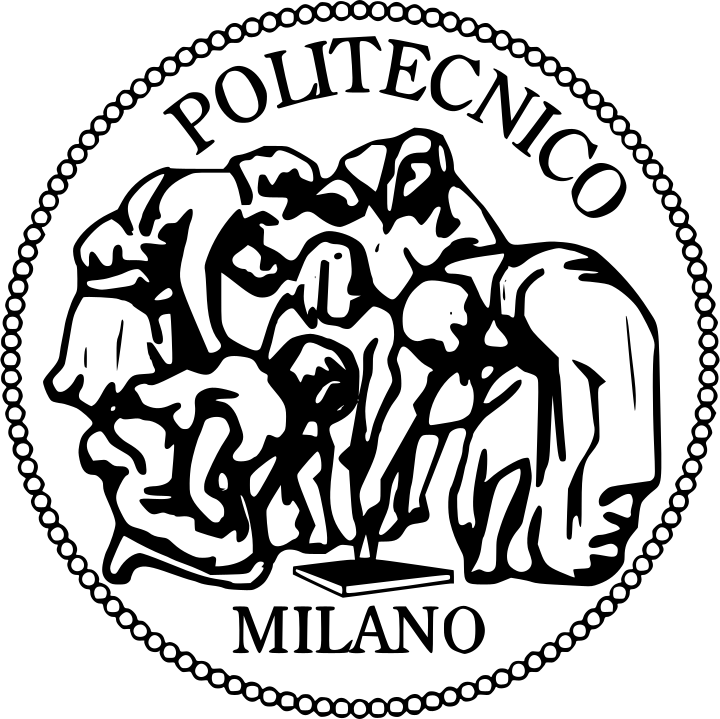
\includegraphics[width=0.3\textwidth]{title-page/logo-polimi}
\end{figure}
\par
\end{center}

%%%%%%%%%% Thesis title goes here!
\begin{center}
\LARGE{\textbf{Consensus based control for a} \\\textbf{Unmanned Aerial Vehicle formation}}
\vspace{1.0cm}
\par
\end{center}

%%%%%%%%%% Advisor and co-advisor names go here!
\begin{flushleft}
\begin{tabular}{ll}
\textbf{Advisor:}      & \textbf{Prof. Marco LOVERA}\tabularnewline
\textbf{Co-Advisors:}  & \textbf{Eng. Pietro PANIZZA}\tabularnewline
                       & \textbf{Eng. Mattia GIURATO}\tabularnewline
\end{tabular}\vspace{0.3cm}
\par
\end{flushleft}

%%%%%%%%%% Student name goes here!
\begin{flushright}
\begin{tabular}{ll}
\textbf{Thesis by:} & \tabularnewline
\textbf{Alex DELBONO} & \textbf{Matr. 850114}\tabularnewline
\end{tabular}\vspace{1cm}
\par
\end{flushright}

\begin{center}
{\large{}\textbf{Academic Year 2016\textendash 2017}}
\par
\end{center}{\large \par}

\end{titlepage}

\restoregeometry

\cleardoublepage{}

%%%%%%%%%%%%%%%%%%%%%%%%%%%%%% Dedication
\begin{flushright}
\emph{A Pietro, una persona vera ed altruista come poche\ldots{}
}
\cleardoublepage{}
\par
\end{flushright}

%%%%%%%%%%%%%%%%%%%%%%%%%%%%%% Acnowledgment
\chapter*{Acknowledgments}
\addcontentsline{toc}{chapter}{Acknowledgments}
%«È di cattivo gusto ringraziare il relatore. Se vi ha aiutato ha fatto solo il suo dovere» Uberto Eco, Come si fa una tesi di laurea


%%%%%%%%%%%%%%%%%%%%%%%%%%%%%% Abstract
\chapter*{Abstract}
\addcontentsline{toc}{chapter}{Abstract}
%The abstract must contain 3 main logic blocks which will be discussed in the introduction.

%Field of work
%The first block must contain a sentence which describes the field of work, and eventually another sentence which focuses the specific objective of the work in details.

%Purpose of the thesis
%The second block must start with the words «The purpose of the thesis is …».

%Short recap
%The last block must summarize the conducted activities and the obtained results (evaluating them eventually).

This thesis is about the synchronized flight of a formation of multirotors which execute a mission.
The mission is characterized by a trajectory for each drone which composes the formation.
The formation must be able to deal with unforeseen events, which can compromise
the outcome of the mission. In order to do that, the drones must exchange information
with each others and a support network is therefore needed.

The purpose of this thesis is to present the algorithm for synchronized formation flight
called consensus algorithm and implement it in a simulated environment
and in a real system with heterogeneous drones. We want to verify that the theoretical
results can be applied in a real distributed system, with not ideal network performances.

In the first part, we explain the algorithm used during the experimental work,
while in the following chapter the software and hardware used are presented.
In the last chapters, we show in detail the structure of the software and the experiment conducted.
In particular, many simulations will be presented to confirm the quality of the
consensus algorithm. Finally, a comparison between the simulated results and the ones
obtained in the real environment is proposed.


%%%%%%%%%%%%%%%%%%%%%%%%%%%%%% Sommario
\chapter*{Sommario}
\addcontentsline{toc}{chapter}{Sommario}
%Il testo delle tesi redatte in lingua straniera dovrà essere introdotto da un ampio estratto in lingua italiana, che andrà collocato dopo l’abstract.

La tesi tratta di volo sincronizzato di una formazione di multirotori che eseguono una missione,
caratterizzata da una traiettoria per ogni drone che compone la formazione.
La formazione deve essere in grado di reagire a eventi inaspettati, che possono
compromettere l'esito della missione stessa.
Per raggiungere tale scopo, i droni devono scambiare informazioni, attraverso
una rete di supporto.

L'obbiettivo della tesi è di presentare l'algoritmo utilizzato per il volo sincronizzato,
chiamato algoritmo di consenso e implementarlo sia in un ambiente simulato,
che in un sistema reale, composto da macchine eterogenee. Si vuole verificare che
i risultati teorici possano essere applicati in un sistema reale distribuito, dotato di
una rete di comunicazione dalle prestazioni non ideali.

Nella prima parte della tesi, verrà esposto l'algoritmo usato durante il lavoro sperimentale,
mentre nel capitolo seguente saranno presentati l'hardware e il software.
Negli ultimi capitoli saranno evidenziati nel dettaglio la struttura del software
e gli esperimenti condotti.
In particolare, saranno mostrate alcune simulazioni, in modo da confermare la bontà
dell'algoritmo di consenso.
Infine, nell'ultimo capitolo, sarà proposta una comparazione tra i risultati
delle simulazioni e quelli ottenuti mediante l'implementazione in un sistema reale.

\tableofcontents

%%%%%%%%%%%%%%%%%%%%%%%%%%%%%% List of figures
\listoffigures
\addcontentsline{toc}{chapter}{List of figures}
\cleardoublepage{}

%%%%%%%%%%%%%%%%%%%%%%%%%%%%%% List of tables
\listoftables
\addcontentsline{toc}{chapter}{List of tables}
\cleardoublepage{}

%%%%%%%%%%%%%%%%%%%%%%%%%%%%%% Introduction
\chapter*{Introduction\label{chap:introduction}}
\addcontentsline{toc}{chapter}{Introduction}
\markboth{Introduction}{Introduction}
%The introduction must be atomic, it does not have to include subsections nor paragraphs.

%The title, the abstract and the introduction must appear as chinese boxes: if read in this order, they must progressively show the informations about the topic in order to catch the attention of the reader.

%The introduction must be divided in three main logic blocks as well:
%General overview
%A brief description of the work
%Structure of the thesis

These years are characterized by the development of the robotics.
The growing applications of mobile robots and drones in many fields
has brought important increasing in the number of robotic vehicles.
Many commercial solutions are available, but in many cases they offer
a product which needs an expert pilot. For this reason and due to the high prices,
the diffusion of mobile robots is limited. In the latest years, these problems were
mitigated and we now see lower prices and easier to use products. This will bring a
growing non professional diffusion of robotic vehicles which, hopefully, will populate
our houses and help us in our life.
The most important application of UAVs are the ones related to exploration and data
collection. Indeed, drones are fundamental in inspection of unknown areas, such as
forests or unreachable terrains.
Also the monitoring of industrial artifacts constitutes a valuable application of UVAs.
For instance, solar panels, wind turbines, high-voltage cables or tubes can be
supervised using aerial vehicles.
The multimedia production is the field in which the drones are most present. Indeed,
most of the machines are equipped with high-definition cameras in order to provide
professional videos.

The power consumptions of the machines are significantly reduced in the last years
and we are now able to build smaller and lighter vehicles.
In particular, in the aerial field, there are commercial products which weight
about 200g with a flight time of 20 minutes.
These improvements allow us to develop more advanced features, such as
trajectory planning, obstacles avoidance, formation flight.
The development of autonomous UAVs is fundamental in application such as humanitarian
response around the world. When a natural calamity happens, the UAVs can play a
crucial role, delivering essential goods or finding missing people. Moreover, the
operations can be done without risking the safety or life of the rescuers, because
they can act remotely or plan an autonomous mission.

The trajectory planning is essential for the development of autonomous vehicles,
because the generation of a feasible trajectory for a mission is a requirement,
otherwise no mission can be done.
The trajectory generation is an hard problem, because of its computational complexity.
Indeed, many suboptimal algorithm have been developed in order to reduce the
complexity.
There are different classes of planning algorithm and they can be summarized as follows:
\begin{itemize}
  \item Artificial Potential Field: these algorithms assigns a value of the potential
  for every point in the map. The goal has the lowest (highest) value and the obstacles
  have high (low) values. Then, the robot tries to descend (climb) the potential,
  in order to reach the goal.

  \item Sampling Based Planning: random samples are used to find a path from the
  starting point to the goal. Advanced random samples techniques can be used in order
  to reduce the complexity of the algorithm.

  \item Grid Based Planning: these kind of algorithm overlay a grid on the map, so
  every configuration corresponds with a grid pixel.
  The robot can move from one grid pixel to any adjacent grid pixels as long
  as that grid pixel does not contain an obstacle.

  \item Reward-Based Planning: the robot can apply different actions in every state
  of the world. The outcome of an action can be not deterministic and after every
  action, the robot gains a reward. The objective of the robot is to maximize the
  sum of the rewards.
\end{itemize}

Another important aspect is the obstacle avoidance. The trajectory usually is planned
offline, when the mission is not started yet. So, the trajectory does not take into
account the fact that an unplanned obstacle might interfere with the mission. In this
case another algorithm is implemented in order to run online. This kind of algorithms
are called obstacle avoidance algorithms and they replan locally the trajectory, in
order to get rid of unforeseen events. These algorithms need the drone to be equipped
with proximity sensors, which provide information about the surrounding environment.
Different methodologies have been developed for obstacles avoidance. The main ones are
summarized below without details.

\begin{itemize}
  \item Artificial Potential Field: as before, the idea of this approach is that
  obstacles exert a virtual repulsive force, given by the potential field, to push
  away the robot from them and the goal position generates a virtual attractive
  force to guide the robot to it.

  \item Virtual Force Field method (VFF): is the combination of the Artificial Potential
  Field with the concept of Probabilistic Occupancy Grid maps.

  \item Fuzzy Controller for Obstacle Avoidance: as the name says, a fuzzy controller
  is used to derives the variable for the vehicle’s orientation and acceleration,
  depending on the current perception of the robot’s sensors

  \item Vector Field Histogram method (VFH): improved version of the VFF method.

  \item VFH+, VFH$^*$ method: improved versions of the VFH method, but more computational costly.
  The most recent one is the VFH method, which uses an A$^*$ search.

  \item Traversability Field Histogram (TFH): The local path planner bases on
  the VFH concept but is extended by the information provided within the Traversability Map.

  \item Dynamic Window Approach: the algorithm takes into account the dynamic and kinematic constraints
  of the robot and it is similar to the VFH+ algorithm. The method is called
  dynamic window approach and considers only admissible velocities which can be
  reached within the next time interval and which allow the robot to stop safely.

  \item Curvature Velocity Space method: This method chooses a point in the linear-angular
  velocity space which satisfies some constraints and maximizes an objective function.
  This objective function tries to move the robot close to the commanded direction at
  the highest feasible speed, while travelling the trajectory with the largest clearance from obstacles.

  \item Beam Curvature method: improvement for the curvature velocity space method.

  \item Nearness diagram Navigation: it is similar to the VFH method, but uses
  a polar histogram to derive actions to be taken for the robot.
\end{itemize}

When multiple machines have to fly in a formation, a synchronization mechanism is
needed. Indeed, if one of the drones has to deviate from the planned trajectory
(for instance, because of an unplanned obstacle), the formation must be preserved.
To reach the synchronization, the vehicles must communicate with each others and
exchange information.
Notions from graph theory are needed to analyze the behaviour of the system
and demonstrate the convergence properties.

This work is focused on the presentation of a distributed synchronization algorithm,
which we call "Consensus Algorithm". Every drones must exchange its mission progression
with its neighbors and must adjust its mission progression based on the information
received from the other vehicles.
The algorithm is a distributed algorithm and it is executed on every vehicles.


In the first chapter, we will show the theoretical aspects of the of the "Consensus Algorithm".
Then, we will provide a general overview of the hardware and software used to deploy the algorithm.
In the third chapter we will show the software implementation of the main part of the
system, providing classes and snippets of code.
At the end, we will explain in the fourth and fifth chapters the simulated and experimental results of
our work. We will apply the algorithm to a real system and we will present our results and its
performances.


%%%%%%%%%%%%%%%%%%%%%%%%%%%%%% Chapter 1
\chapter{State of the art\label{chap:state_of_the_art}}
%%Introduction of the chapter
The literature about the "Consensus" is grown significantly in the latest years
because of the increasing presence of autonomous vehicles. This, in accordance with
the new improvements in robotics, has brought a growing interest in consensus
between multiple agents which have to accomplish a mission in cooperative or adversarial
scenarios.

The "Consensus" theory takes its roots in Graph Theory and Automatics and it can
be used to coordinate a mission in order to achieve the synchronization between
the vehicles even when there might be some unforeseens which force one or more
components of the mission to change the planned trajectory or task. In this case,
the other components identify this variation and they will act for preserving the
synchronization.

The "Consensus" algorithm is a distributed algorithm which sometimes can be simulated
in a centralized fashion because of the reduced computational power of the machines
involved in the mission, which are equipped with low power hardware to account for
the crucial issue of power consumption.
In this scenario, a centralized server simulates the algorithm and communicates with
all the machines.

The most common "Consensus" application is a spatial and timing consensus.
Each vehicle of the formation has to travel along a specified trajectory and the
completion of the mission occurs when all the agents reach the final positions of their
spatial paths. The algorithm has to guarantee the difference between
the ending time at which all the vehicles finish their tasks is minimized and
asymptotically goes to zero when the execution time goes to infinity and no other
unforeseen happens.
We also consider formations of Unmanned Aerial Vehicles but the key concepts can
be freely applied to other categories of robots when they are able to follow a trajectory.
This study is focused on this kind of application and further
simulation result and experimental achievements are presented in the chapters
\ref{chap:simulation_results} and \ref{chap:experimental_results}.

In the following we refer to the main work of Venanzio Cichella in this field \cite{cichellaMain}
in order to provide an homogeneous state of the art about the "Consensus".
The paper considers all the details needed to build a "Consensus" system.
We can identify the main components of this kind of systems:
\begin{itemize}
  \item Parametrized trajectory
  \item Virtual time
  \item Consensus law
  \item Network topology
\end{itemize}



%% Sections of the chapter
\section{Parametrized trajectory\label{sec:parametrized_trajectory}}
The trajectory is a spatial path with associated a timing law and it is used
to identify position and orientation of the center of mass of our agent in the space.
We can start with the following definition of a generic trajectory $ p_{d,i}(t_d) $
for $ N $ vehicles:

\begin{equation}  \label{eq:traj_def}
  p_{d,i}:[0,t^f_{d,i}] \rightarrow \mathbb{R}^3, \quad i = 1,2,\dots,N
\end{equation}
where $ t_d \in [0, T_d] $, with $T_d := max \{ t^f_{d,1}, \dots , t^f_{d,N} \} $,
is the time variable of the trajectory, while $ t^f_{d,i} \in \mathbb{R}^+ $
are the individual final mission times of the vehicles obtaining during the planning
phase. Usually all this final times are equal and therefore
$ t^f_{d,1} = \dots = t^f_{d,N} = T_d$, but we introduced the notation
for the sake of completeness.
Obviously the trajectories need to be collision free and must satisfy spatial
and temporal constraints due to the dimension of the vehicle and its maximum
velocities and accelerations.

We now parametrize the trajectory using a dimensionless variable $ \zeta_i \in [0,1]$,
related to the time $t_d$. In this way we can specify a function $ \theta( \cdot )$,
which represents the timing law associated with the spatial path $p_{d,i}(\zeta_i)$.
We can specify this timing law using the dynamic relation of the form:

\begin{equation}  \label{eq:tim_law_def}
  \theta( t_d ) = \frac{d \zeta_i}{dt_d}
\end{equation}

where $ \theta( t_d ) $ is a smooth and positive (the parameter increases when
the time increases) function.

It is desirable that an analytical expression for the function $ \zeta_i (t_d) $
to be available, since it allows a one-to-one correspondence between the time
variable $t_d$ and the parameter $ \zeta_i $.
Using the timing law, defined in \eqref{eq:tim_law_def}, the map $ \zeta_i ( t_d) $
is given by the integral:

\begin{equation}  \label{eq:zeta_law_def}
  \zeta( t_d ) = \int^{t_d}_0 \theta_i(\tau) d \tau
\end{equation}

Usually, all this functions are defined as polynomials in order to make quicker and
easier the evaluation process, since multiplication and addition are the basic
operations in a digital processor, but it is not mandatory to use them and a
generic shape for the functions can be designed.
We have defined all the elements of a trajectory and we do not enter in details
about the trajectory generation phase.
Further details about boundary conditions and flyable trajectory which satisfy
the dynamic constraints of the vehicles can be found in \cite{cichellaMain} and
are extensively presented in \cite{trajGeneration1}, \cite{trajGeneration2},
\cite{trajGeneration3}.


\section{Virtual time\label{sec:virtual_time}}

Given $ N $ collision free trajectories, we want each vehicle to follow a \textit{virtual target},
moving along the path computed offline by the trajectory generation algorithm.
The objective can be achieved introducing a \textit{virtual time}, $ \gamma_i $,
which is used to evaluate the trajectory and can be adjusted online to reach
the synchronization even when external disturbances occur.
Thus, the position of the $ i^{th} $ virtual target is denoted by $ p_{d,i} ( \gamma_i (t))$
and the $ i^{th} $ vehicle tries to follow it, by reducing to zero a suitably defined
error vector using control inputs.

Considering the trajectory $ p_{d,i} (t_d) $ produced by the trajectory generation
algorithm, we consider the virtual time $ \gamma_i $ as a function of time $ t $,
which relates the actual time $t$ to mission planning time $t_d$.

\begin{equation}  \label{eq:virt_time_func}
  \gamma_i : \mathbb{R}^+ \rightarrow [0, T_d], \qquad for \; all \quad i = 1,2,\dots,N
\end{equation}

We can now define the virtual target's position, velocity and acceleration, which
have to be followed by the $ i^{th}$ vehicle at time $t$

\begin{equation}  \label{eq:pos_vel_acc_def}
  \begin{aligned}
  p_{c,i}(t) = \ & p_{d,i}(\gamma_i(t)) \\
  v_{c,i}(t) = \ & \dot{p}_{d,i} (\gamma_i(t), \dot{\gamma}_i (t)) \\
  a_{c,i}(t) = \ & \ddot{p}_{d,i} (\gamma_i(t), \dot{\gamma}_i(t), \ddot{\gamma}_i(t))
  \end{aligned}
\end{equation}

With the above formulation, if $ \dot{\gamma} = 1$, then the speed profile of
the virtual target is equal to the desired speed profile computed at trajectory
generation level.
Indeed, if $ \dot{\gamma} = 1$, for all $t \in [0, T_d]$, with $\gamma_i(0) = 0$,
it implies that $\gamma_i(t) = t_d$ for all $t$ and thus:

\begin{equation*}
  p_{c,i}(t) = p_{d,i}(\gamma_i(t)) = p_{d,i}(t) = p_{d,i} (t_d)
\end{equation*}

In this particular case, the desired and commanded trajectories coincide
in every time instant and also the velocity profiles coincide with the ones
chosen at the trajectory generation time.
If instead $\dot{\gamma_i} > 1$, it implies a faster execution of the mission;
on the other hand, $\dot{\gamma_i} < 1$ implies a slower one.

We can now normalize $\gamma_i$ in order to have a range which is $[0,1]$. We simply
need to divide all by $T_d$. In this way, we could use Bezier curves in order to
represent the spatial path. This kind of curves offer interesting properties for
computing minimum distances between two of them and allow the computation of
smooth trajectories. In any case, it is not mandatory to use them and a general
function could be used instead.

The second order derivative of $\gamma_i$, $\ddot{\gamma}_i$, is a free parameter
used to achieve the consensus. In the next section we will introduce the control law
which commands its evolution during time and we will explain how it is possible to
implement a distributed algorithm.


\section{Consensus law\label{sec:consensus_law}}

Now, we formally state the path following problem. We define as $p_i(t) \in \mathbb{R}^3$
the position of the center of mass of the $i^{th}$ agent and since $p_{c,i}(t)$
describes the commanded position to be followed by the agent at time $t$, the errors
are defined as:

\begin{equation}  \label{eq:pos_vel_acc_err}
  \begin{aligned}
  e_{p,i}(t) = \ & p_{c,i}(t) - p_i(t) \in  \mathbb{R}^3\\
  e_{v,i}(t) = \ & v_{c,i}(t) - \dot{p}_i(t) \in  \mathbb{R}^3
  \end{aligned}
\end{equation}

Then, the objective reduces to that of regulating the error defined in \eqref{eq:pos_vel_acc_err}
to a neighbourhood of zero.
This task is solved with an autopilot capable of following the set points computed
from the desired trajectory at specified instances of time.

The virtual time is the parameter used to reach consensus between multiple vehicles.
In fact, since the the trajectories are parametrized by $\gamma_i$, the agents are
synchronized at time $t$ when:

\begin{equation} \label{eq:diff_gamma}
  \gamma_i(t) - \gamma_j(t) = 0 \quad for \; all \quad i,j \in {1 , \dots , N}, \quad i \neq j
\end{equation}

We can also control the rate of progression of the mission using a parameter
$\dot{\gamma}_d \in \mathbb{R}$, which represents the velocity of the virtual time
with respect to the real time. All the agents share this variable and they proceed
at the same rate of progression if:

\begin{equation} \label{eq:diff_dot_gamma}
  \dot{\gamma}_i(t) - \dot{\gamma}_d(t) = 0 \quad for \; all \quad i \in {1 , \dots , N}
\end{equation}

Adjusting $\dot{\gamma}_d$ we can decide the speed of the mission: for instance
if we set $\dot{\gamma}_d = 1$ and \eqref{eq:diff_gamma} and \eqref{eq:diff_dot_gamma}
are satisfied for all the vehicles, then the mission is executed at the speed
originally planned in the trajectory generation phase.
If instead we use $\dot{\gamma}_d > 1$ or $\dot{\gamma}_d < 1$ we carry out the
mission faster or slower.
This term can be changed in real time in order to get rid of moving objects or
unplanned obstacles which force to change one of the path of the agents.
For the purpose of "Consensus", the parameter is only a reference command,
rather than a control input.

Now we introduce the coordination control law which regulates the evolution of
$\ddot{\gamma}_i(t)$ during the time and determines $\gamma_i(t)$:

\begin{equation} \label{eq:cons_law}
  \begin{aligned}
    \ddot{\gamma}_i(t) = & \; \ddot{\gamma}_d(t) - b (\dot{\gamma}_i(t) - \dot{\gamma}_d(t)) - a \sum_{j \in \aleph_i} (\gamma_i(t) - \gamma_j(t)) - \overline{\alpha}_i (e_{p,i}(t)) \\
    \dot{\gamma}_i(0) = & \; \dot{\gamma}_d(0) = 1 \\
    \gamma_i(0) = & \; \gamma_d(0) = 0
  \end{aligned}
\end{equation}
where $a$ and $b$ are positive coordination control gains, while $\overline{\alpha}_i (e_{p,i}(t)$
is defined as:

\begin{equation} \label{eq:error_term}
  \overline{\alpha}_i (e_{p,i}(t)) = \frac{v_{c,i}^T(t) e_{p,i}(t)}{||v_{c,i}(t)|| + \epsilon}
\end{equation}

with $\epsilon$ being a positive design parameter and $e_{p,i}$ the position
error vector defined in \eqref{eq:pos_vel_acc_err}.
In the equation \eqref{eq:cons_law} we have four terms. The feedforward term
$\ddot{\gamma}_d$ allows the virtual target to follow the acceleration profile of
$\gamma_d$.
The second term $- b (\dot{\gamma}_i(t) - \dot{\gamma}_d(t))$ reduces the error
between the speed profile imposed by $\dot{\gamma}_d(t)$ and $\dot{\gamma}_i(t)$,
which corresponds to the control objective given in \eqref{eq:diff_dot_gamma}.
In particular, if $\dot{\gamma}_d(t)$ is one, then the virtual target converges
to the desired speed profile chosen in the trajectory generation phase.
The third term $- a \sum_{j \in \aleph_i} (\gamma_i(t) - \gamma_j(t))$ ensures that
all the vehicles are coordinated with their neighbors as specified in \eqref{eq:diff_gamma}.
Finally, the fourth term $- \overline{\alpha}_i (e_{p,i}(t))$ is a correction term
used to take into account for the path following errors of the agent. Indeed if the
vehicle is behind its target, the term is not zero and the target slows down in order
to wait the real vehicle.

With this control law we want our vehicles to be synchronized and to proceed at
a desired rate of progression, in order to accomplish the mission even when
some unforeseen disturbances occur during the execution phase.


\section{Network topology\label{sec:network_topology}}



%%%%%%%%%%%%%%%%%%%%%%%%%%%%%% Chapter 2
\chapter{Theoretical results\label{chap:theoretical_results}}
\input{chapters/chapter-02/theoretical_results.tex}

%%%%%%%%%%%%%%%%%%%%%%%%%%%%%% Chapter 3
\chapter{System architecture\label{chap:system_architecture}}
In this chapter, we will describe the hardware and software architecture of the system.
Most of the software is completely decoupled from the hardware part and can be run
on different machines, allowing portability and reusability. On the contrary, the
code is developed only for the specific hardware; mostly the code which is more related
to the specific functionalities of the hardware itself. We will have an overview of the hardware
used and then we will show a general software architecture and its deployment on the
machines involved.

%% Sections of the chapter
\section{Hardware}

The hardware used to run the system is heterogeneous and we will show in details
the machines involved in the project.

First of all, we used a desktop pc as a ground station. It specifics are listed below:
\begin{itemize}
  \item Processor: Intel Core(TM) i5-6500 CPU @ 3.20GHz
  \item Memory: 16 GB
  \item Network: Intel Gigabit CT Network Adapter
  \item Storage: 230 GB
\end{itemize}

On this machine, we run a virtual machine which has the following specifics:
\begin{itemize}
  \item Processor: 1 Core
  \item Memory: 4 GB
  \item Storage 25 GB
  \item Network: Virtual adapter
\end{itemize}

The flying machines involved in the mission are of two kinds, but both adopt the
same general configuration, even with different hardware. Indeed, they are equipped
with a flight control unit connected with a companion microcomputer by the serial port
The microcomputer communicates with the ground station using the Wifi.

\subsection{Pixfalcon}
The flight control unit adopted it the Pixfalcon (figure \ref{fig:hardware_pixfalcon})
which belongs to the family of the Pixhawk \cite{pixhawk}.

\begin{figure}[h]
\centering
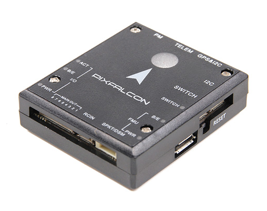
\includegraphics[width=0.35\textwidth]{chapters/chapter-03/figures/hardware_pixfalcon.png}
\caption{Pixfalcon board}
\label{fig:hardware_pixfalcon}
\end{figure}

Its specifications are the following:
\begin{itemize}
  \item Main System-on-Chip: STM32F427
        \begin{itemize}
          \item CPU: 180 MHz ARM Cortex M4 with single-precision FPU
          \item RAM: 256 KB SRAM (L1)
        \end{itemize}

  \item Failsafe System-on-Chip: STM32F100
        \begin{itemize}
          \item CPU: 24 MHz ARM Cortex M3
          \item RAM: 8 KB SRAM
        \end{itemize}

  \item Wifi: ESP8266 external
  \item GPS: U-Blox 7/8 (Hobbyking) / U-Blox 6 (3D Robotics)
  \item Connectivity:
    \begin{itemize}
      \item 1x I2C
      \item 1x CAN (2x optional)
      \item 1x ADC
      \item 4x UART (2x with flow control)
      \item 1x Console
      \item 8x PWM with manual override
      \item 6x PWM / GPIO / PWM input
      \item S.BUS / PPM / Spektrum input
      \item S.BUS output
    \end{itemize}
\end{itemize}

\subsection{Intel Edison}
The companion computers are of two types.
The first kind is the Intel Edison \cite{edison} (figure \ref{fig:hardware_edison})
which is a general purpose computer.

\begin{figure}[h]
\centering
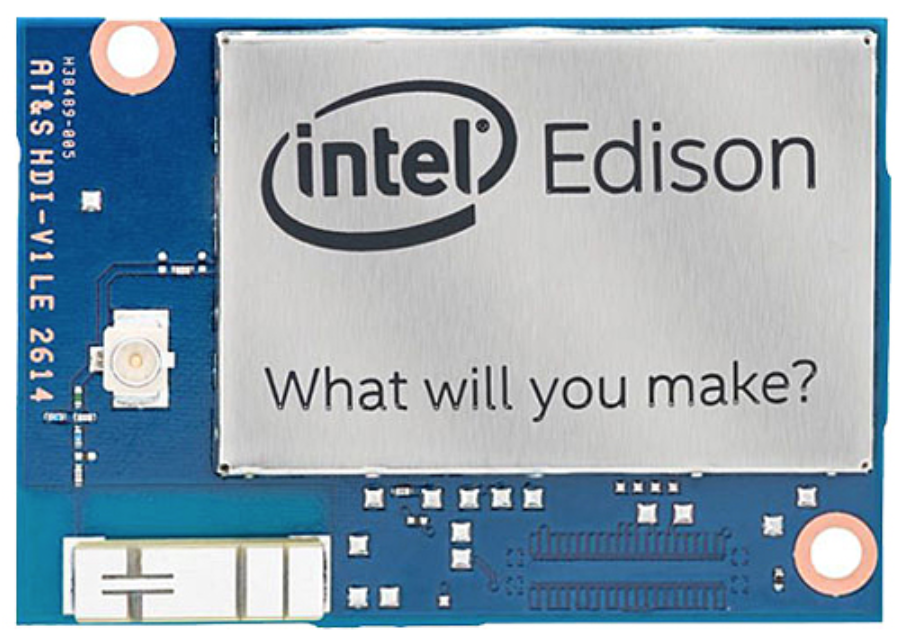
\includegraphics[width=0.35\textwidth]{chapters/chapter-03/figures/hardware_edison.png}
\caption{Edison board}
\label{fig:hardware_edison}
\end{figure}

The specifications are the following:

\begin{itemize}
  \item Atom 2-Core (Silvermont) x86 @ 500 MHz
  \item Memory: LPDDR3 1 GB
  \item Storage: 4 GB EMMC
\end{itemize}

\subsection{RaspberryPi Zero}
The second kind of companion is the RaspberryPi Zero \cite{raspberry}
(figure \ref{fig:hardware_raspberry}).

\begin{figure}[h]
\centering
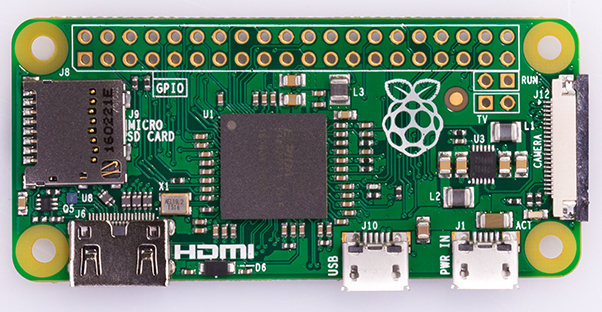
\includegraphics[width=0.35\textwidth]{chapters/chapter-03/figures/hardware_raspberry.jpg}
\caption{RaspberryPi Zero board}
\label{fig:hardware_raspberry}
\end{figure}

The specifications are the following:

\begin{itemize}
  \item Processor:
        \begin{itemize}
          \item Broadcom BCM2835
          \item contains an ARM1176JZFS (ARM11 using an ARMv6-architecture core)
        \end{itemize}

  \item Memory: 512MB LPDDR2 SDRAM

  \item USB On-The-Go port
  \item Mini HDMI
  \item 40pin GPIO header
  \item CSI camera connector (newer version from May 2016)
\end{itemize}

\subsection{Motive Optitrack}
The motion capture system is Motive Optitrack \cite{optitrack}.
We use eight Optitrack Prime 13 cameras \cite{prime13},
arranged on a square as show in the figure \ref{fig:camera_square}.

\begin{figure}[h]
\centering
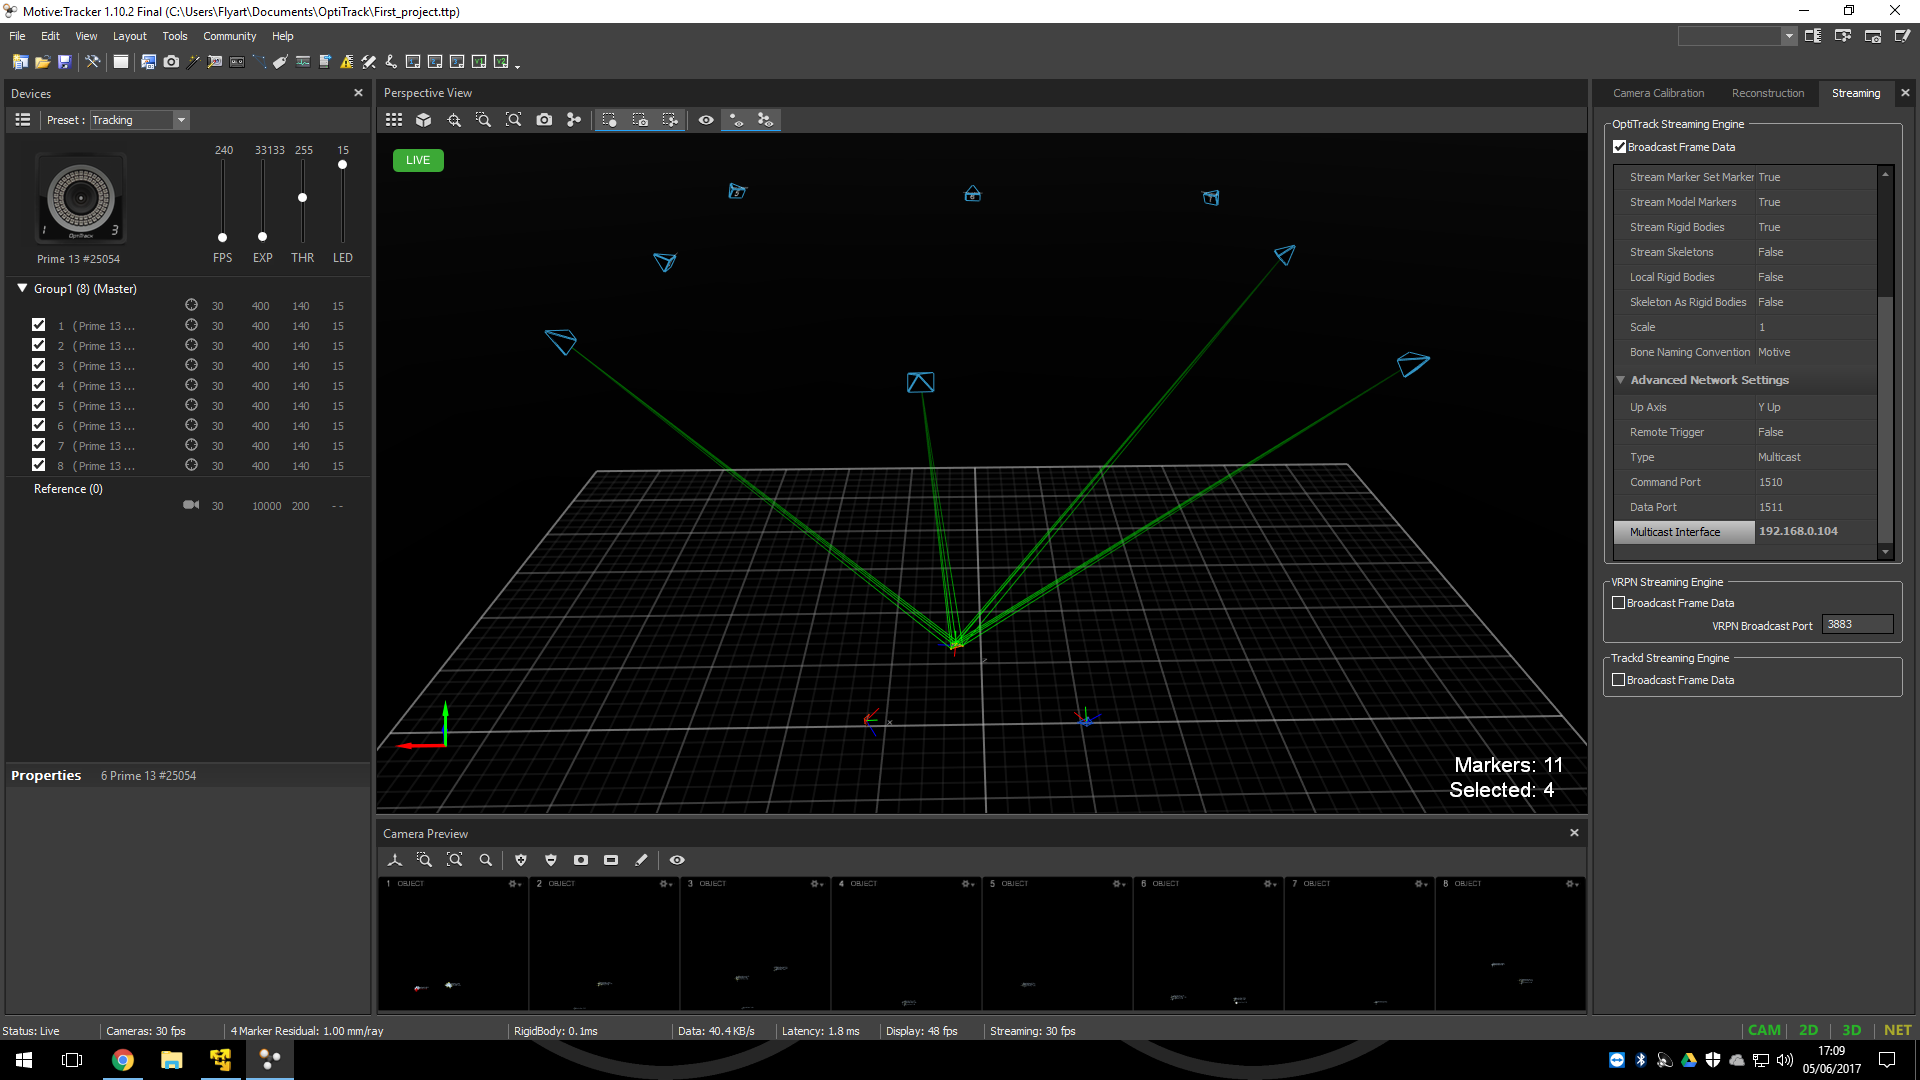
\includegraphics[width=1.0\textwidth]{chapters/chapter-03/figures/cameras_square.png}
\caption{Motive Optitrack screenshot}
\label{fig:camera_square}
\end{figure}

The cameras are connected to a Netgear Prosafe 28PT GE POE \cite{netgear} switch using
Gigabit Ethernet cables.

In order to be visible by the Optitrack system, every drone must be equipped with
markers (figure \ref{fig:marker}), with different configurations,
which make possible the diversification of all the drones. %TODO photo markers

\begin{figure}[h]
\centering
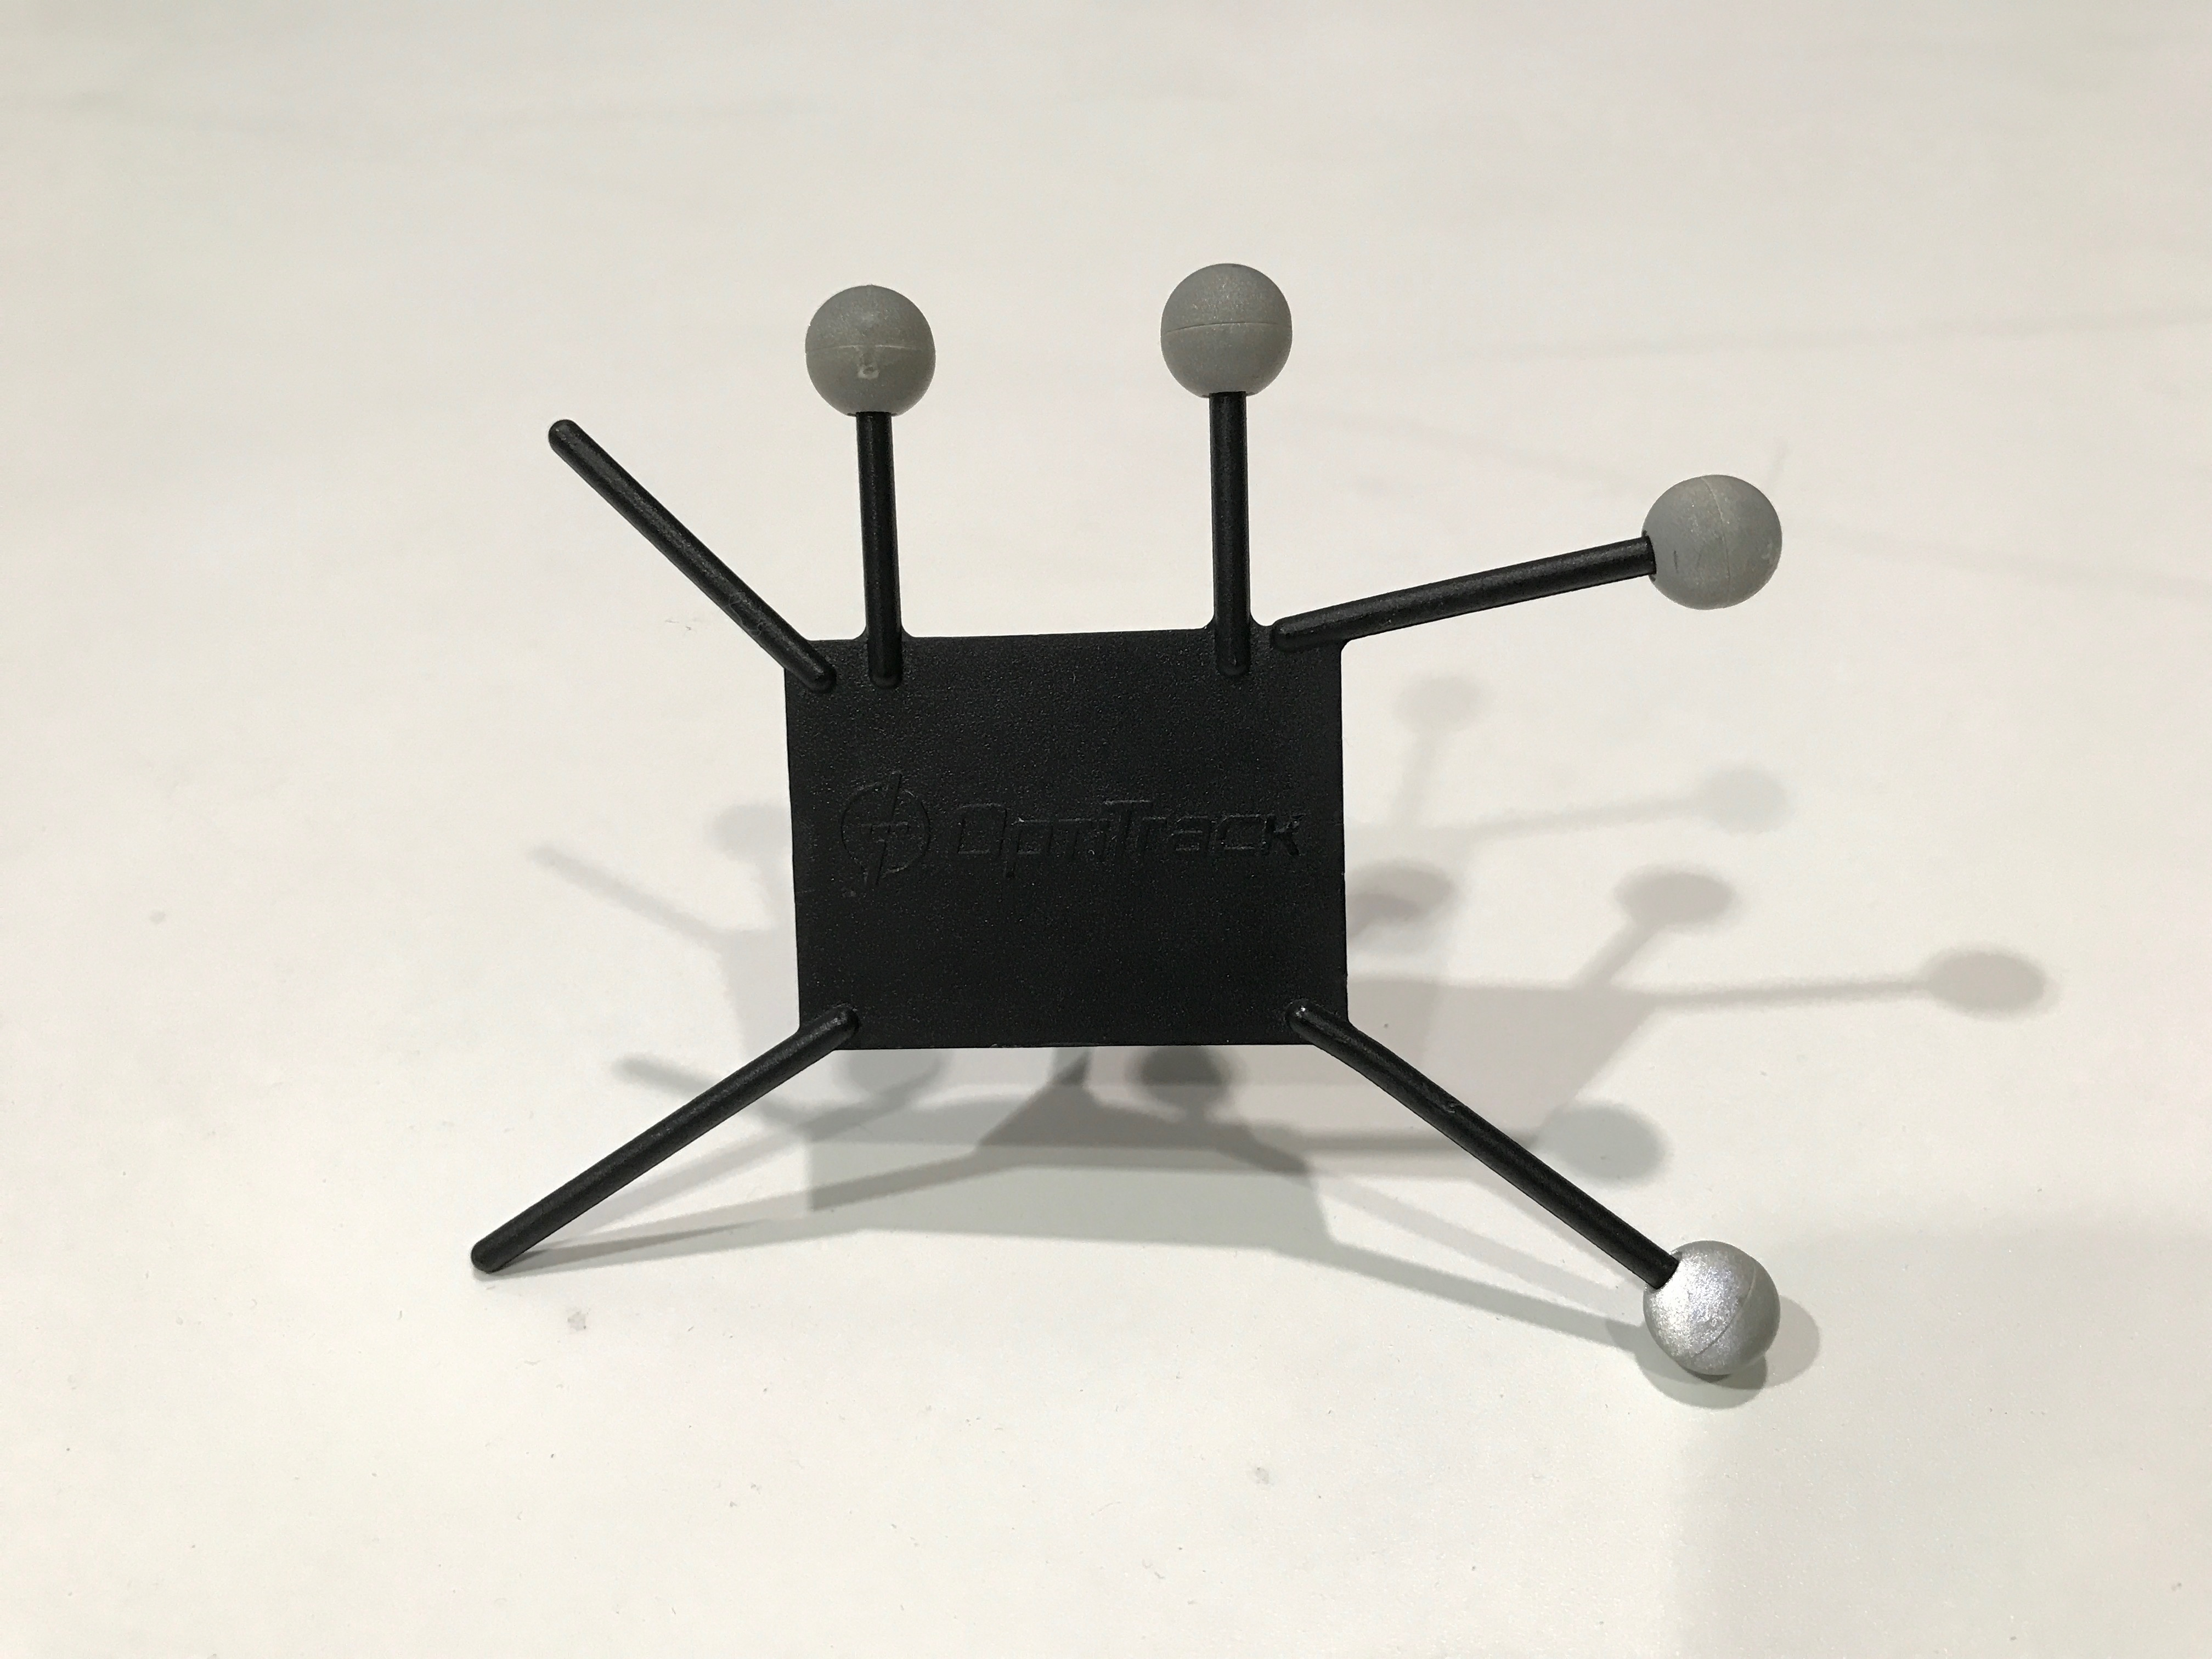
\includegraphics[width=0.7\textwidth]{chapters/chapter-03/figures/marker.jpg}
\caption{Optitrack marker}
\label{fig:marker}
\end{figure}

The two models of drone which we will use are presented in the figures \ref{fig:ant1}
and \ref{fig:hexa}. The first one is the Ant model, which is equipped with the Raspberry
Pi Zero and the Pixfalcon. It is a tiny drones which weights about 200g.
The second one is the Hexa model. It is provided with the Intel Edison board and
the Pixfalcon. It is larger and its diameters is about 40cm long.
As we can see from the figures, the Ant model has four propellers, while the Hexa
is provided with six ones.

\begin{figure}[!htb]
\minipage{0.5\textwidth}
  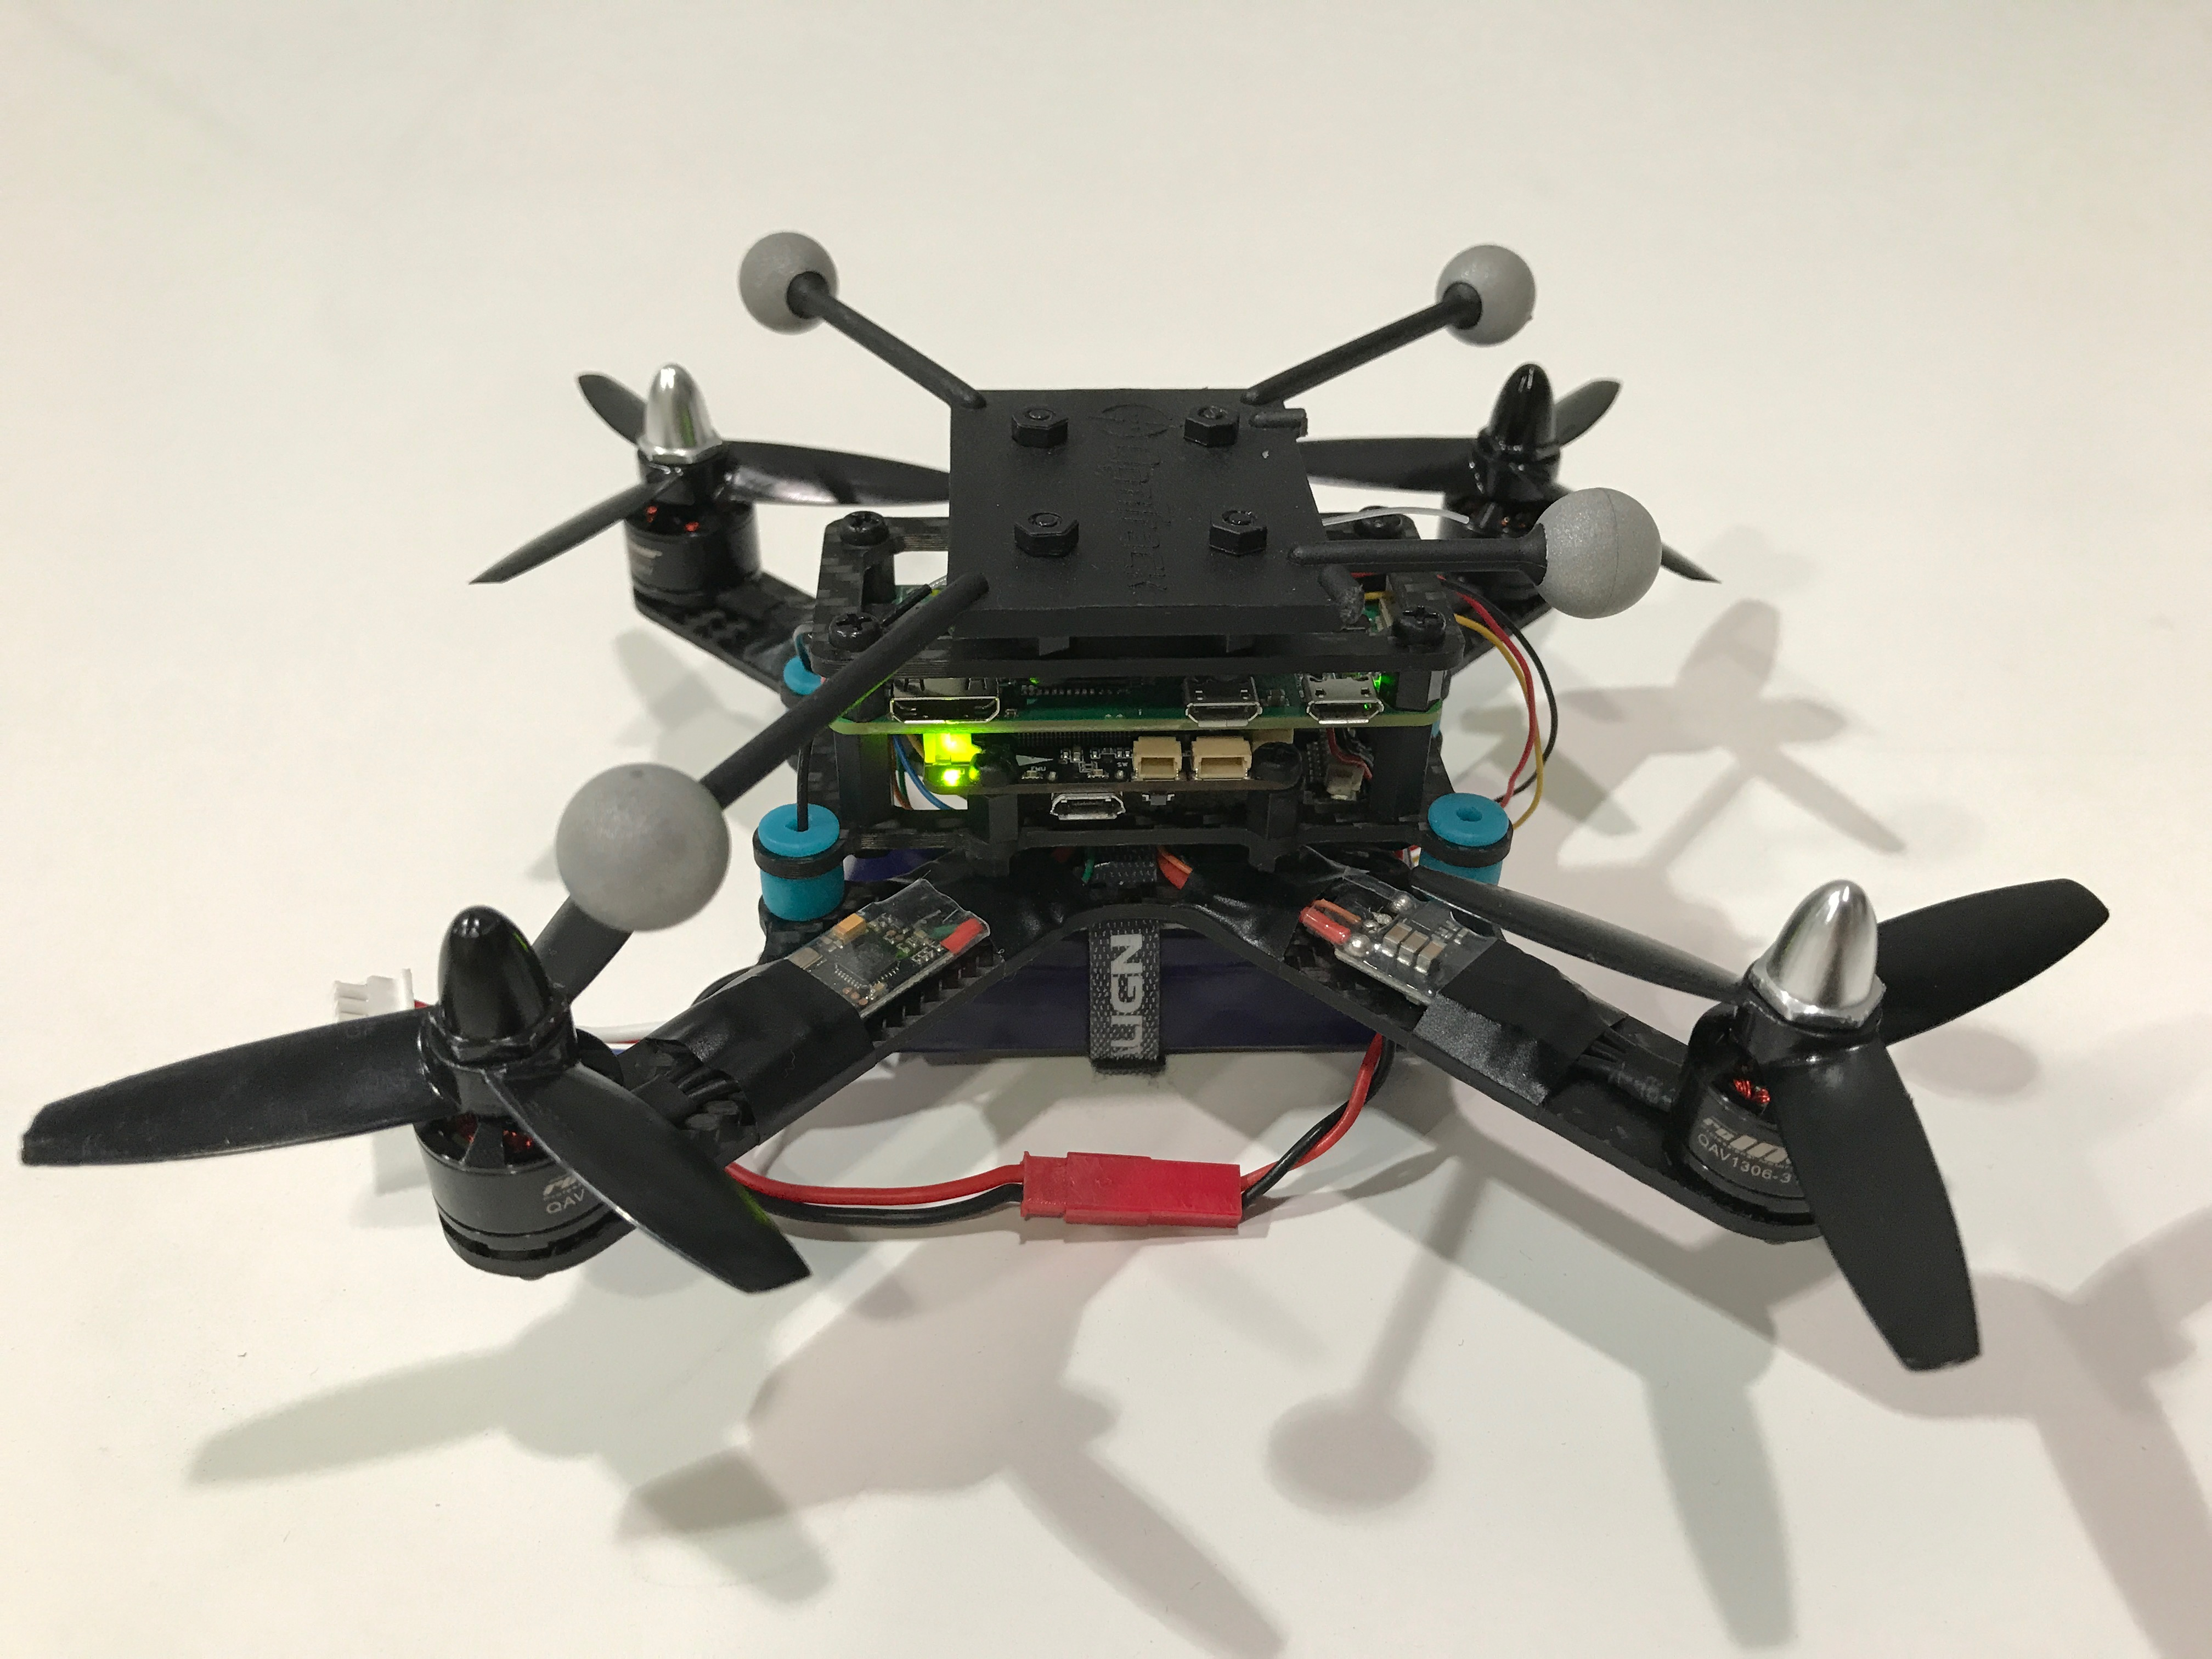
\includegraphics[width=\linewidth]{chapters/chapter-03/figures/ant1_1.jpg}
\endminipage\hfill
\minipage{0.5\textwidth}
  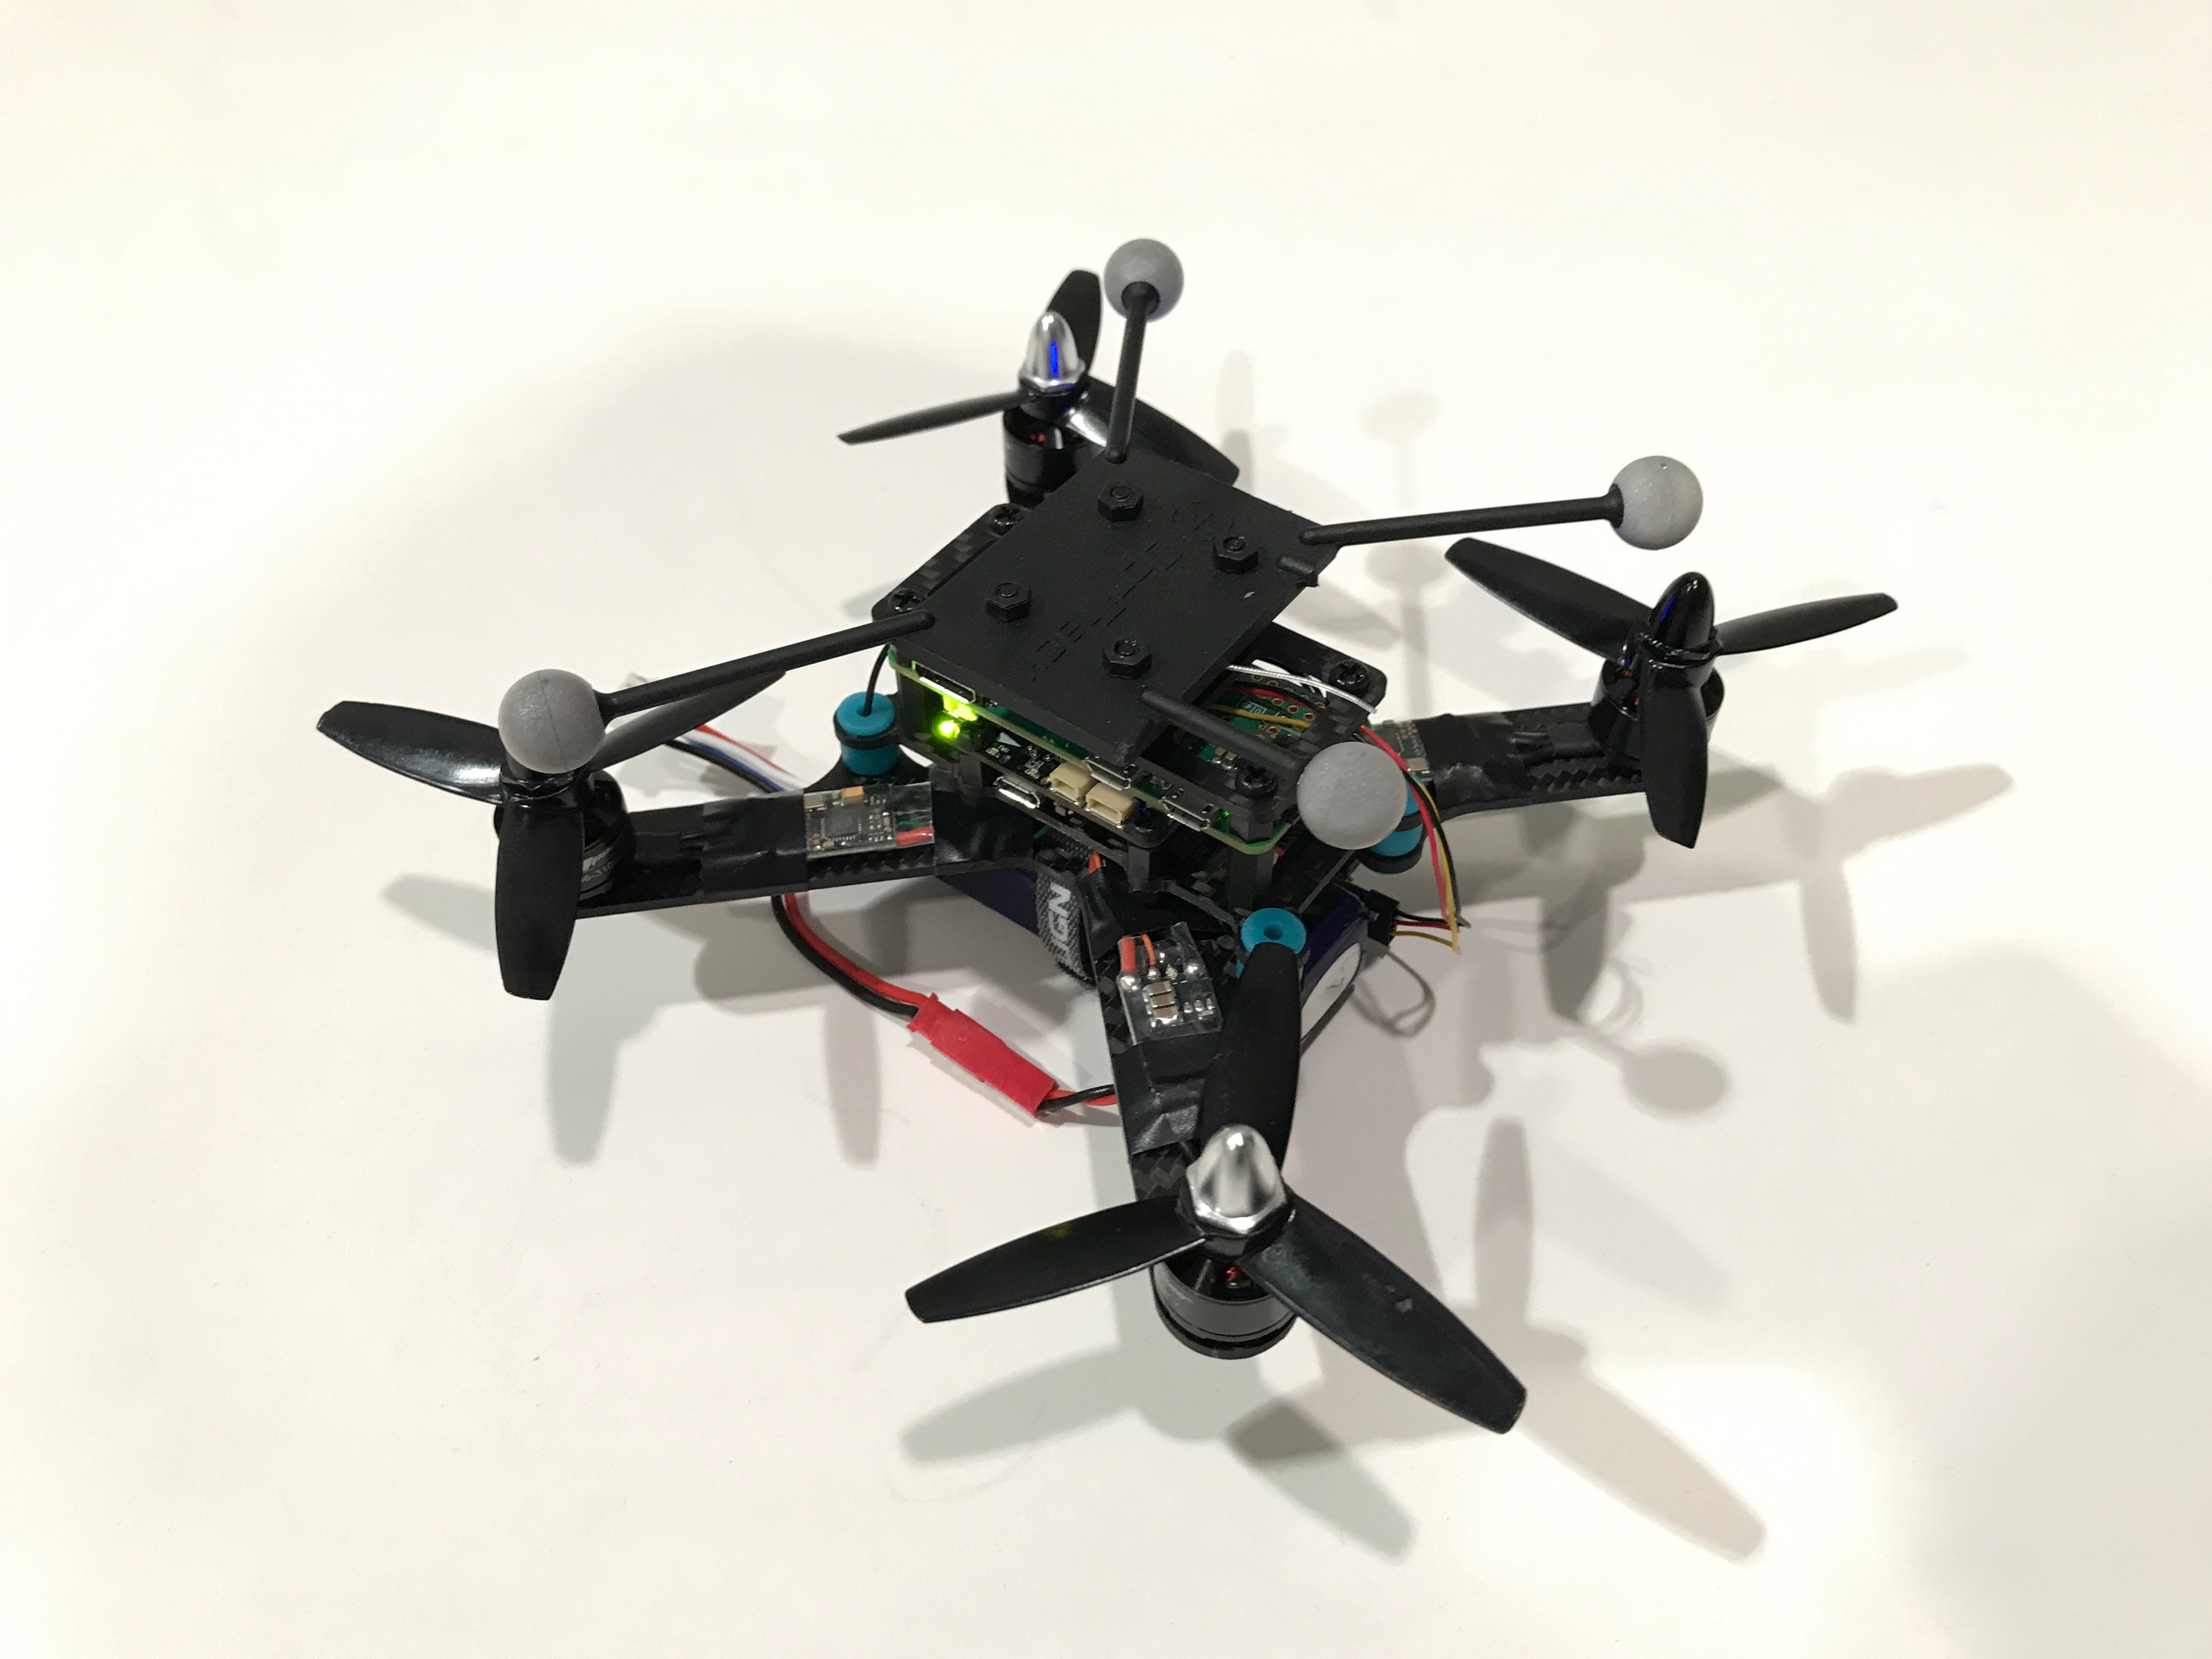
\includegraphics[width=\linewidth]{chapters/chapter-03/figures/ant1_2.jpg}
\endminipage
\caption{Ant drone}
\label{fig:ant1}
\end{figure}

\begin{figure}[!htb]
\minipage{0.5\textwidth}
  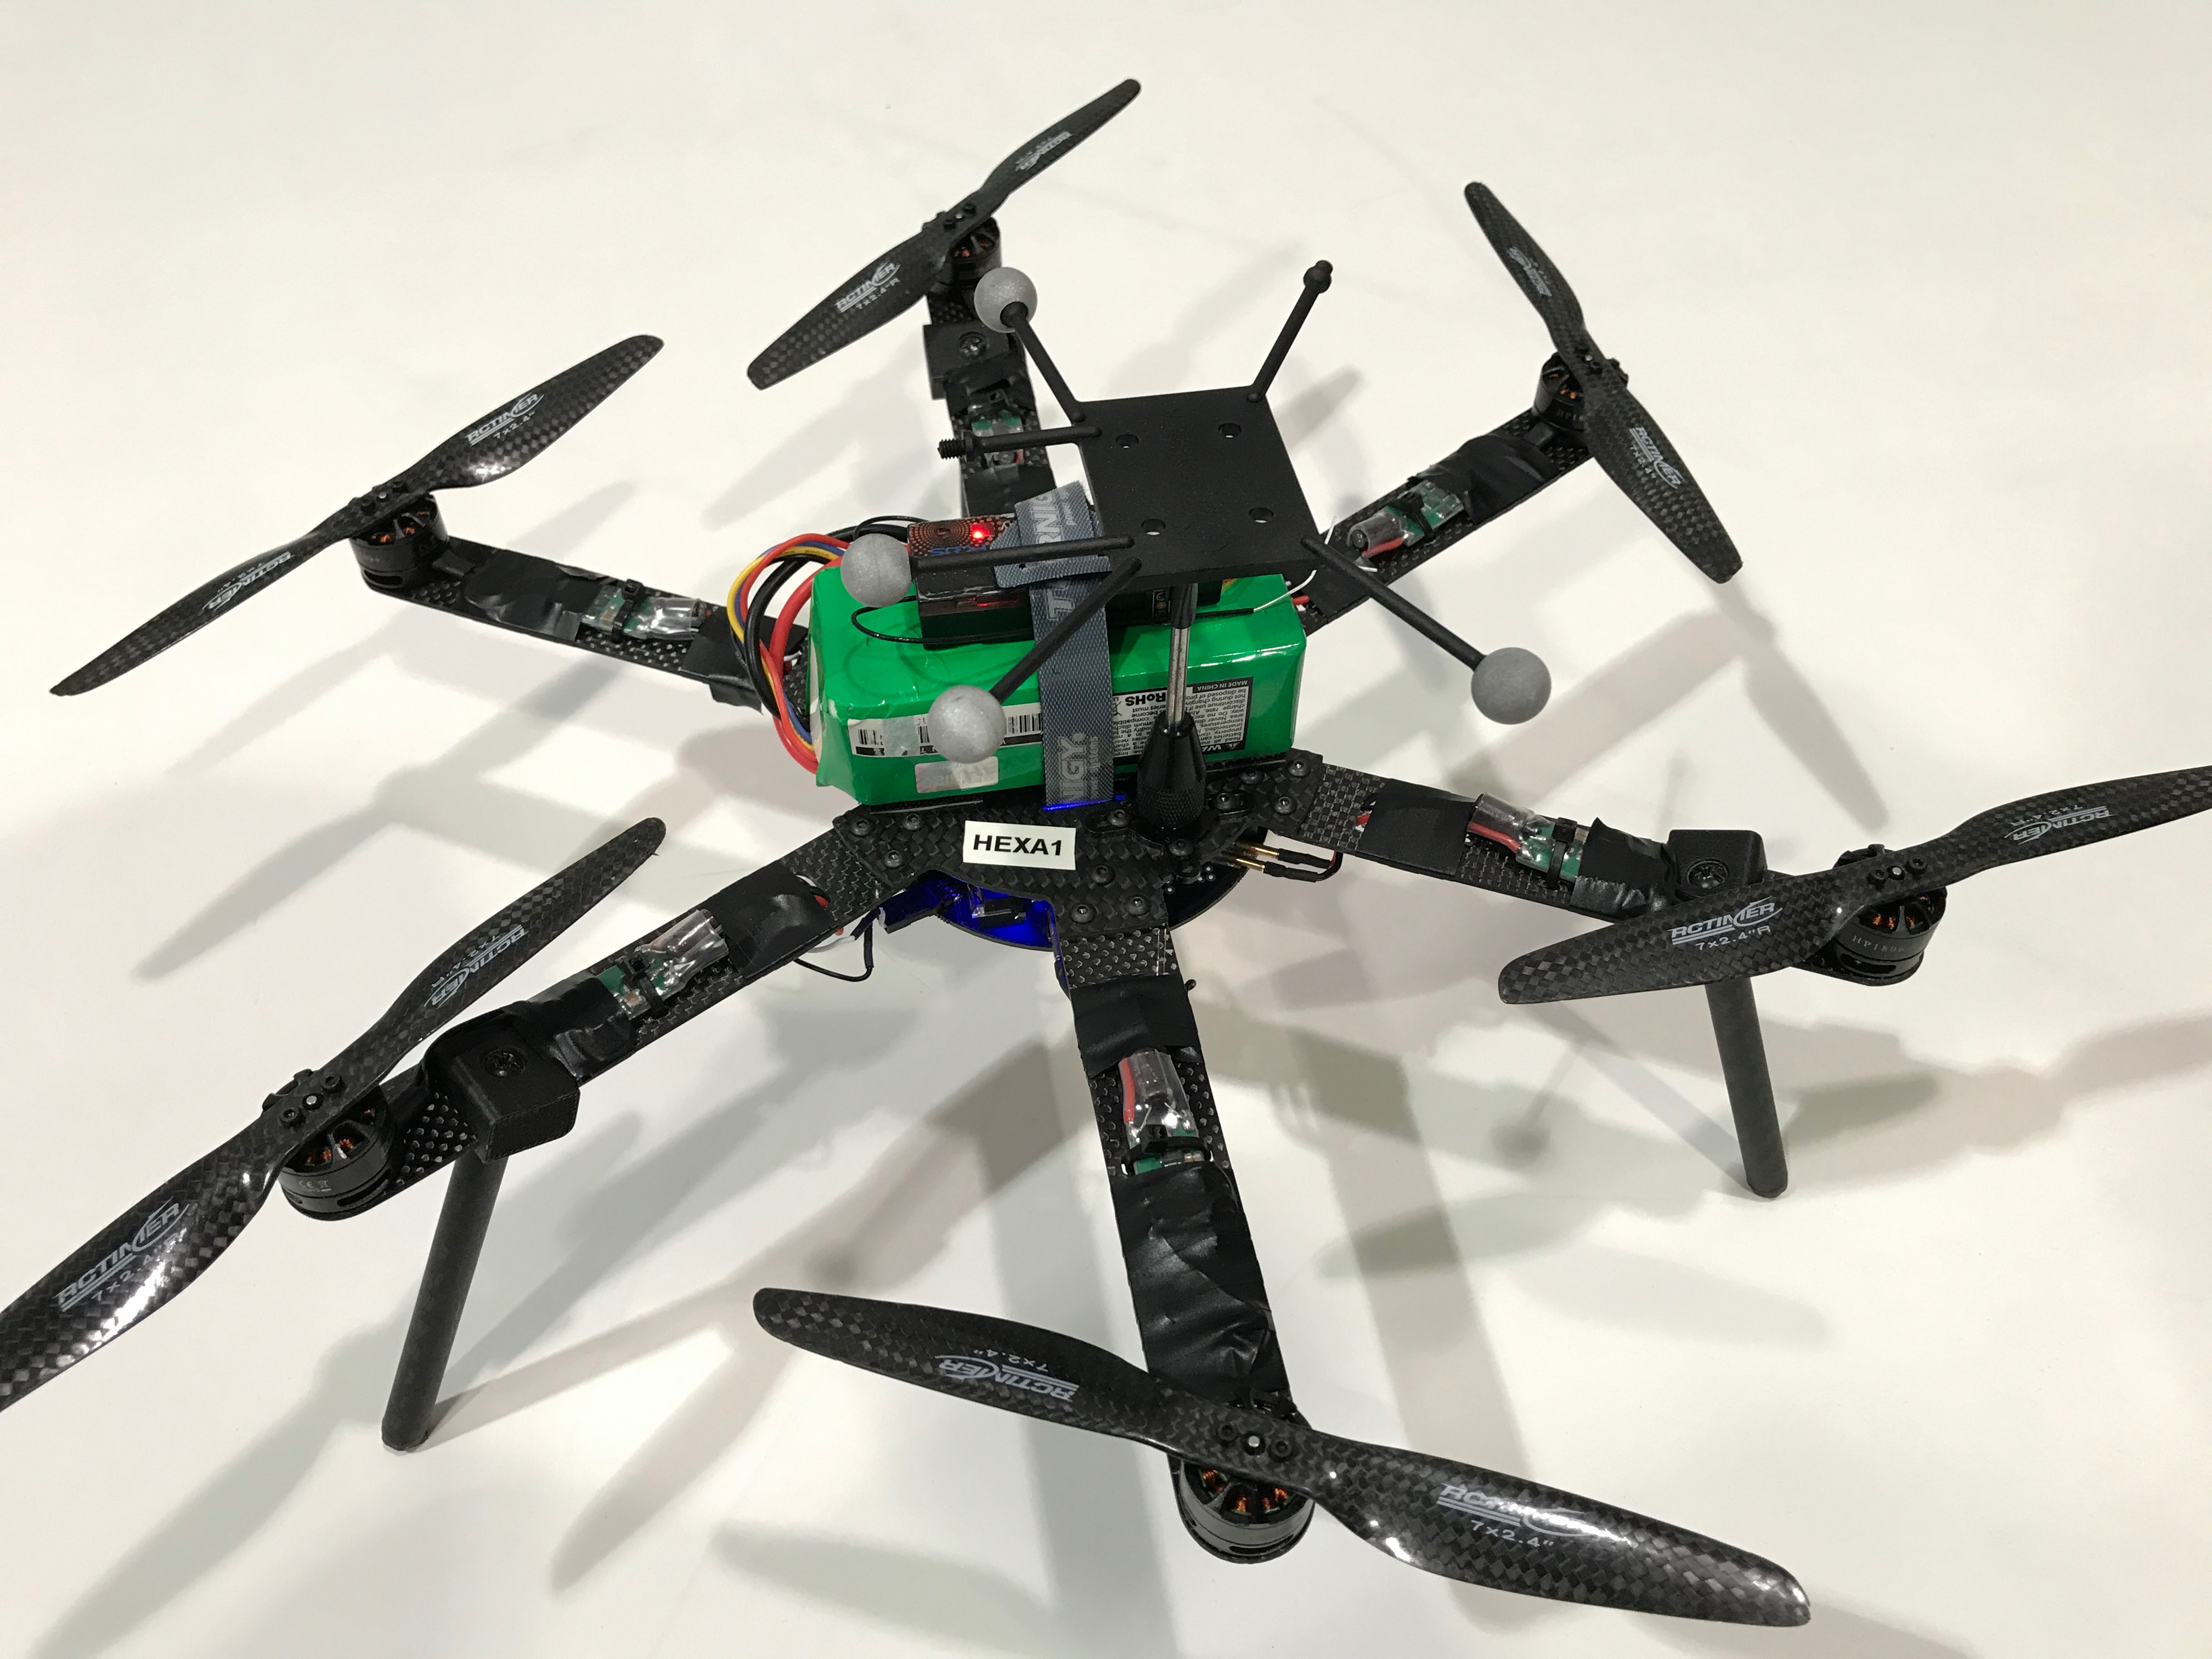
\includegraphics[width=\linewidth]{chapters/chapter-03/figures/hexa_1.jpg}
\endminipage\hfill
\minipage{0.5\textwidth}
  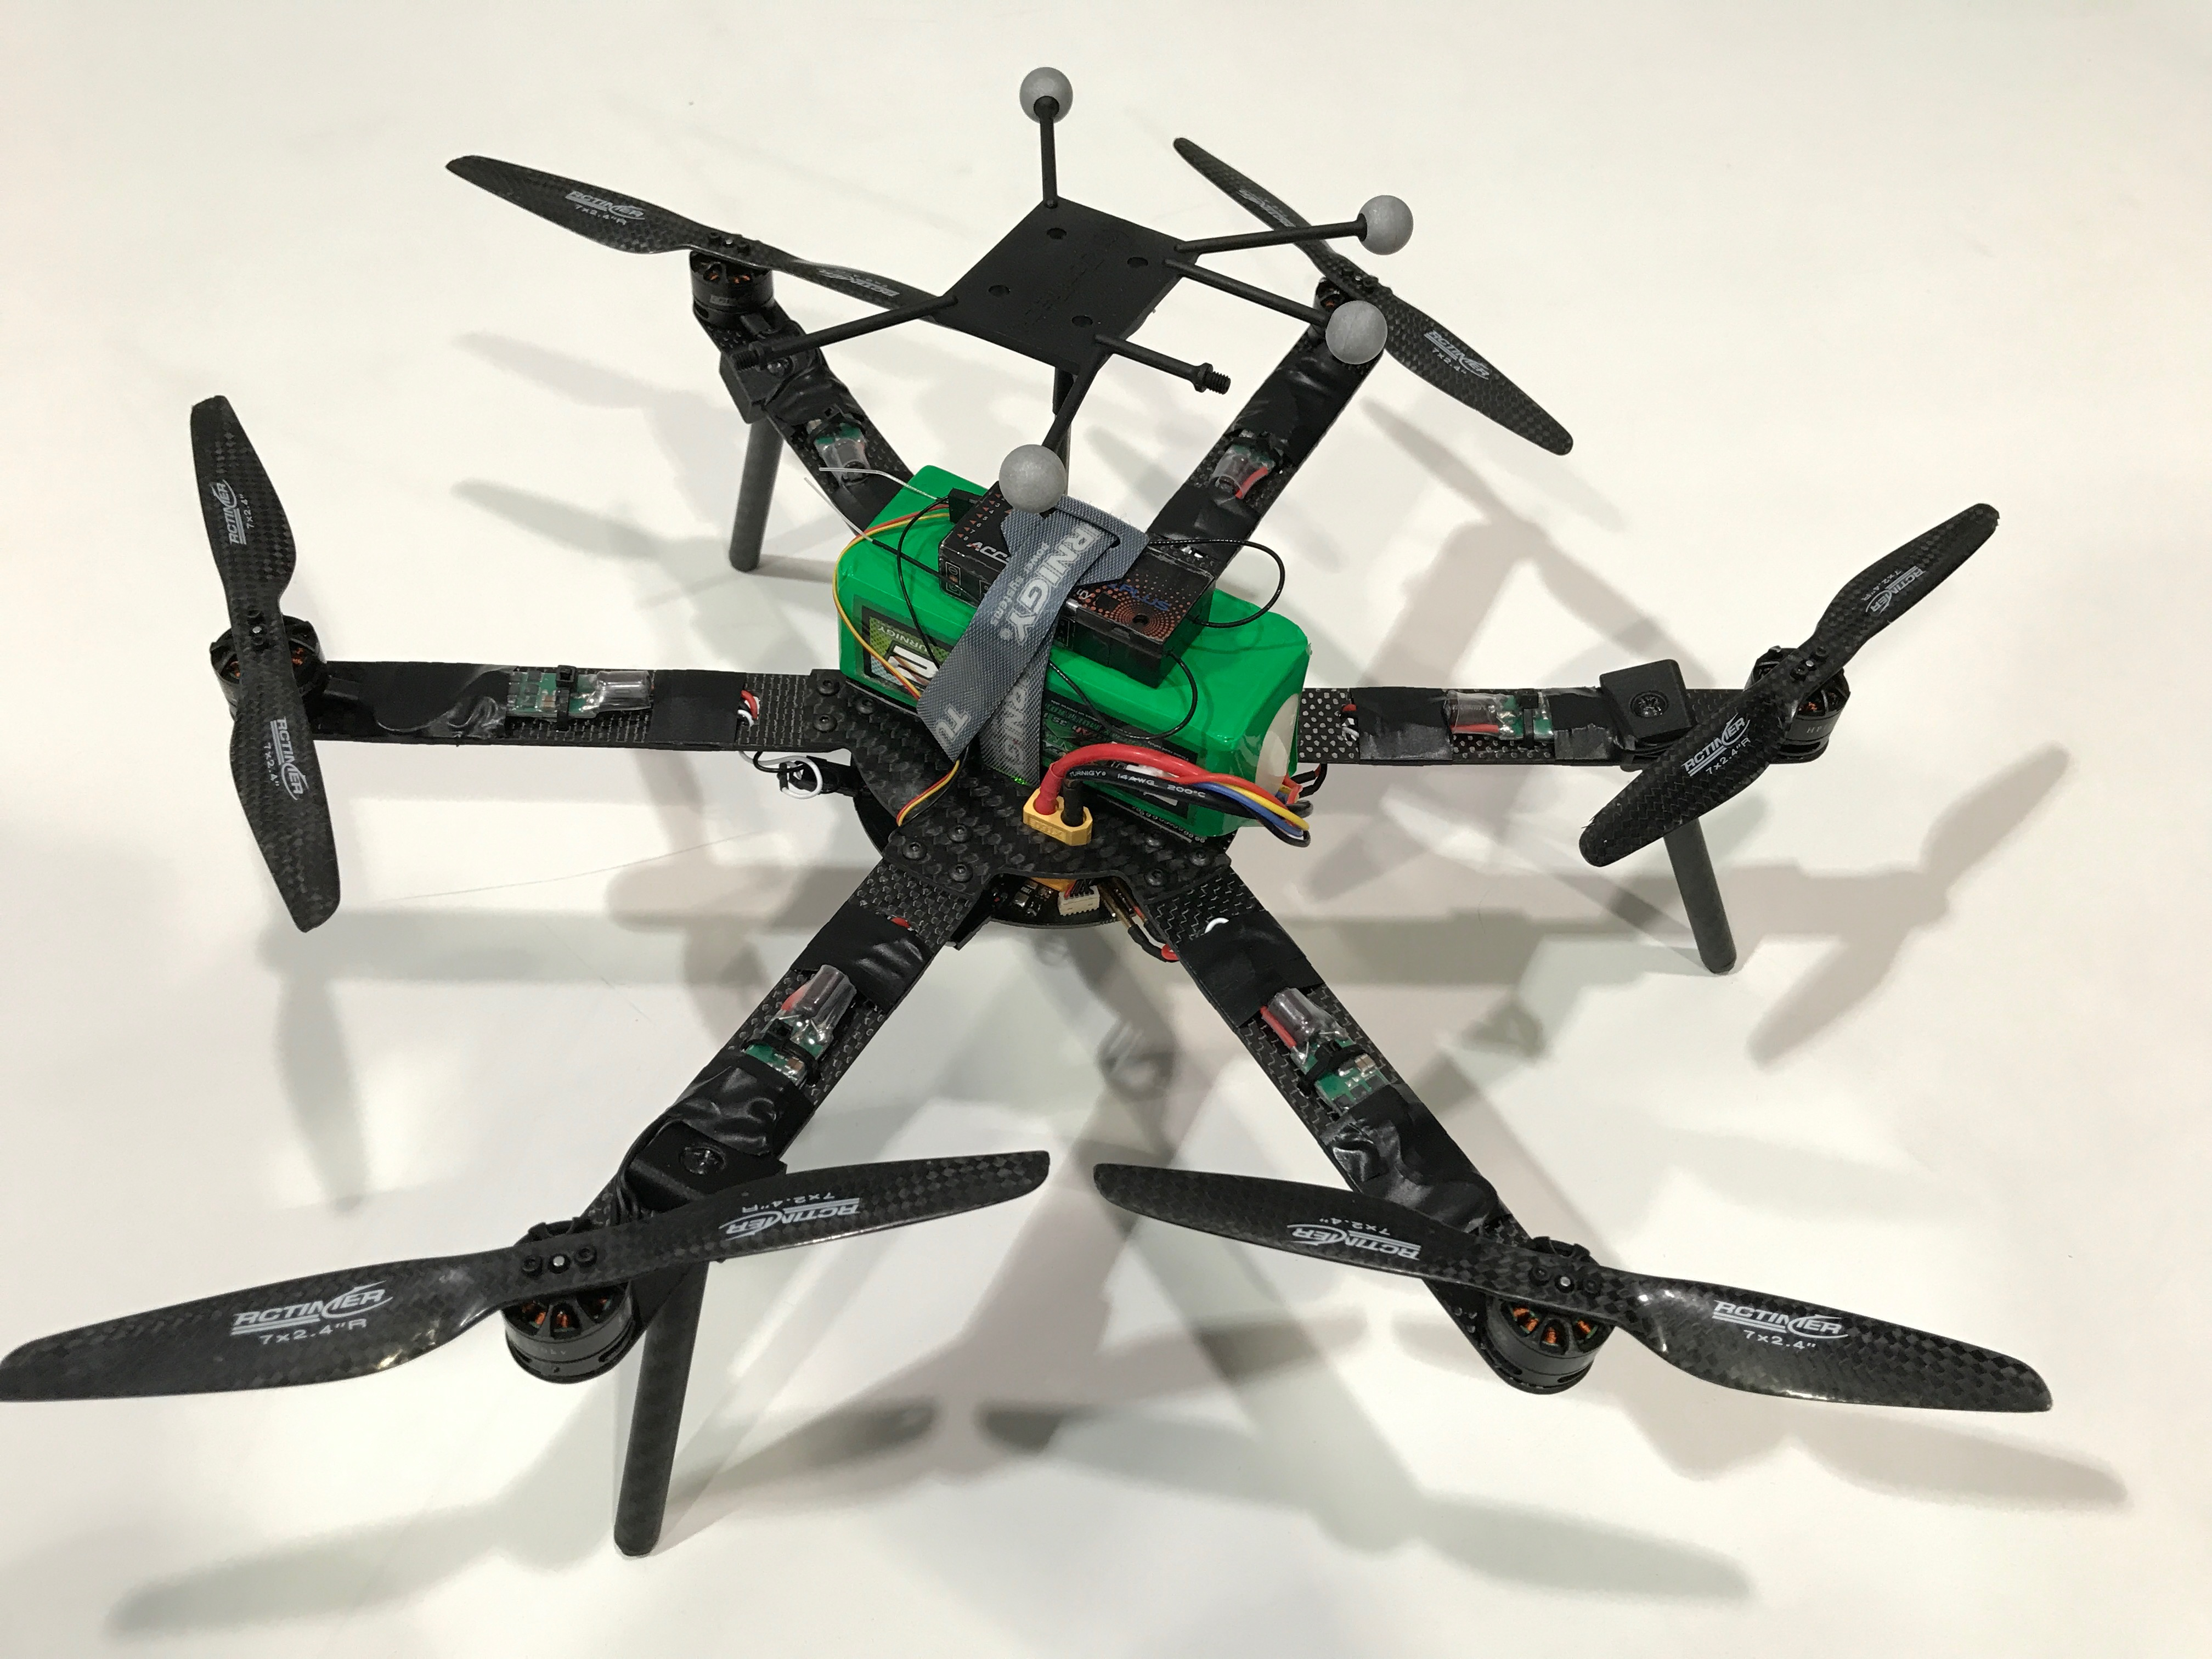
\includegraphics[width=\linewidth]{chapters/chapter-03/figures/hexa_2.jpg}
\endminipage
\caption{Hexa drone}
\label{fig:hexa}
\end{figure}


\section{Software}

We now list all the software adopted in order to execute the algorithm
in a real environment and in the simulated one.

The principal software used to manage the distributed architecture is ROS Kinetic
Kame \cite{ros}.
ROS is a robotic middleware which can manage in a distributed environment more
machines with a structure which is mainly publisher-subscriber.
The central part of the ROS architecture is a node called ROS core, which manages
the topics of the system and the subscriptions.
The ROS core offers also other functionalities such as the Parameter Server or the
possibility to advertise services.
The Parameter Server is a central infrastructure which is responsible for storing
configuration parameters loaded by the nodes of the system.
These parameters can be retrieved by the nodes and used whether needed.
Instead, a ROS service is a sort of remote function call. One node can advertise
the service, which can be called by any other nodes. The call is synchronous and
so the caller is blocked until the callee has executed its callback function.
ROS architecture is based on queues and threads and most of the provided functions
hide part of the implementations of these tools.


\subsection{Ground station}
The ground station runs Windows 10 Pro \cite{windows} and the software used to virtualize a
Desktop machine is VMware \cite{vmware}.
On the virtual machine is installed Ubuntu 16.04 LTS \cite{ubuntu} in order to run software
needed and available only for Unix systems.

On Windows operative system we launch the Motive Optitrack software \cite{optitrack},
which allows to calibrate and control the cameras. It also provides the streaming of
the positions of the markers identified by the cameras and sends it to the Ubuntu
operative system.
Here, the information is converted by a ROS node and sent through the ROS topics,
which are read by the drones. In this way, each drone knows exactly its position.
This node is an open source node called Mocap which can be found on GitHub \cite{mocap}.
On Ubuntu side, we launch the ROS core, which manages all the ROS nodes and topics.

\subsection{Raspberry Pi Zero}
The Raspberry Pi Zero executes a dedicated version of Debian operative system,
which is Raspbian. The version used is Raspbian Jessie 4.4 \cite{raspbian}.

\subsection{Intel Edison}
The Intel Edison runs a version of Debian called Jubilinux version 0.1.1 \cite{jubilinux}.

\subsection{Both companions}
Both companions, the Raspberry and the Edison, are provided with ROS Kinetic and
both have to execute some ROS nodes in order to communicate with the others.

First of all, they run Mavros nodes \cite{mavros}.
This kind of node can be downloaded from GitHub and manages the conversion of the
information taken from the ROS topics to the serial port and vice versa. Indeed,
the ROS messages are converted into Mavlink messages and sent through the serial
to the Pixfalcon autopilot. The same is done for the Mavlink messages from the
autopilot, which are published on ROS topics.

The second kind of ROS node run by the companions, is a custom consensus node, which
loads the desired trajectory and sends the next set point to the Mavros node.
This node will be analyzed in details in the chapter \ref{chap:consensus_node}.

\subsection{Pixfalcon}
The Pixfalcon autopilot is flashed with an open source firmware,
the PX4 Pro Autopilot \cite{px4}, which is downloadable from GitHub.
The release used is the v1.5.5.

\subsection{Additional software}
We use Matlab R2016\_B \cite{matlab} to the data process and to graph plot. We also use it to validate
some theoretical results.

This document is written in  \LaTeX \ \cite{latex} and the code IDE used is Atom \cite{atom},
while the versioning control platform used are GitHub \cite{github} and GitLab \cite{gitlab}.



%%%%%%%%%%%%%%%%%%%%%%%%%%%%%% Chapter 4
\chapter{Cameras setup\label{chap:cameras_setup}}
\input{chapters/chapter-04/cameras_setup.tex}

%%%%%%%%%%%%%%%%%%%%%%%%%%%%%% Chapter 5
\chapter{Drones hardware\label{chap:drones_hardware}}
\input{chapters/chapter-05/drones_hardware.tex}

%%%%%%%%%%%%%%%%%%%%%%%%%%%%%% Chapter 6
\chapter{Drones software\label{chap:drones_software}}
\input{chapters/chapter-06/drones_software.tex}

%%%%%%%%%%%%%%%%%%%%%%%%%%%%%% Chapter 7
\chapter{Trajectories\label{chap:trajectories}}
\input{chapters/chapter-07/trajectories.tex}

%%%%%%%%%%%%%%%%%%%%%%%%%%%%%% Chapter 8
\chapter{Consensus nodes\label{chap:consensus_nodes}}
\input{chapters/chapter-08/consensus_nodes.tex}

%%%%%%%%%%%%%%%%%%%%%%%%%%%%%% Chapter 9
\chapter{Simulation results\label{chap:simulation_results}}
In this chapter we will show the simulations conducted to evaluate the “Consensus
Algotithm”.

As said in the capter \ref{chap:system_architecture}, the software used is Gazebo.
We run SITL (Software in the loop) simulations, through the utilities provided by
the PX4 firmware. Indeed, it provides models of the main topologies of aerial vehicles,
such as plane, VTOL, Tailsitter VTOL and quadrotor.
We will use the quadrotor model called Iris, which can be shown in the picture \ref{fig:iris_model}.

\begin{figure}
\centering
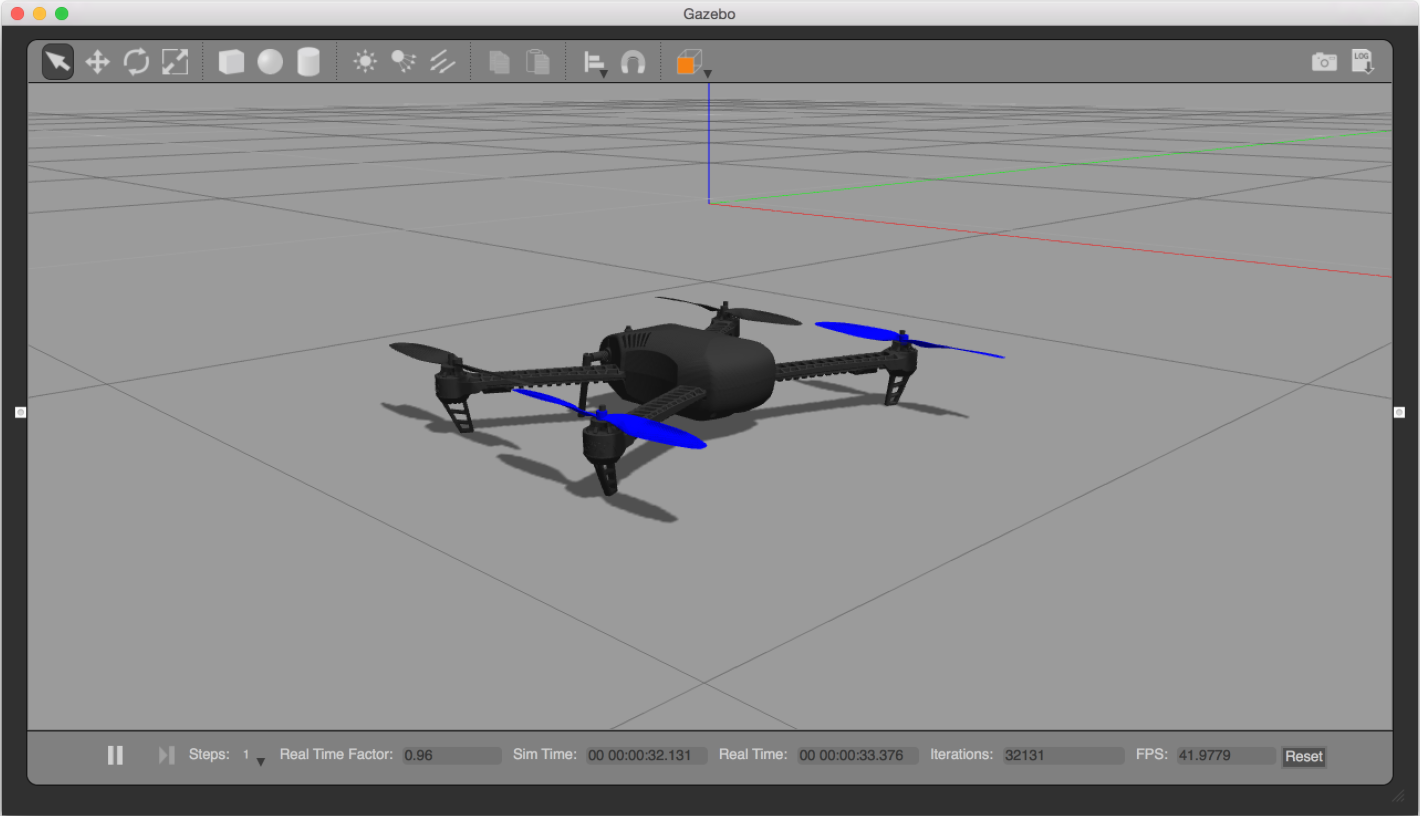
\includegraphics[width=0.9\textwidth]{chapters/chapter-04/figures/iris_model.png}
\caption{Iris model}
\label{fig:iris_model}
\end{figure}

The PX4 firmware is run on a simulated hardware and all the ROS nodes are executed
on the same computer. The physics is simulated by Gazebo and all the components
are interfaced through Gazebo plugins. In this way, the model can interact with
all the external simulated components.

The Gazebo model is specified, using SDF language, in a Gazebo model file.
All the dynamic parameters are listed in this file and also the geometry part
is stated.

The simulations that we will show are of three kinds. First, we present only
the trajectory following problem of a formation of two drones.
In the second simulation, we send a disturbance to one of the drones and we stop it
in its position. Third, we introduce a disturbance which makes one of the drones to
go back following in the reverse order its trajectory.
We see how the “Consensus algorithm” reacts to these disturbances and forces the other
drone to preserve the formation.
We use only two drones because of the computational load of the simulation, but the
concept can be extended freely to an arbitrary number of drones.

\section{Trajectory following}

The simulation is composed by two drones and the trajectory of the mission is shown
in \ref{fig:trajectory}.

\begin{figure}
\centering
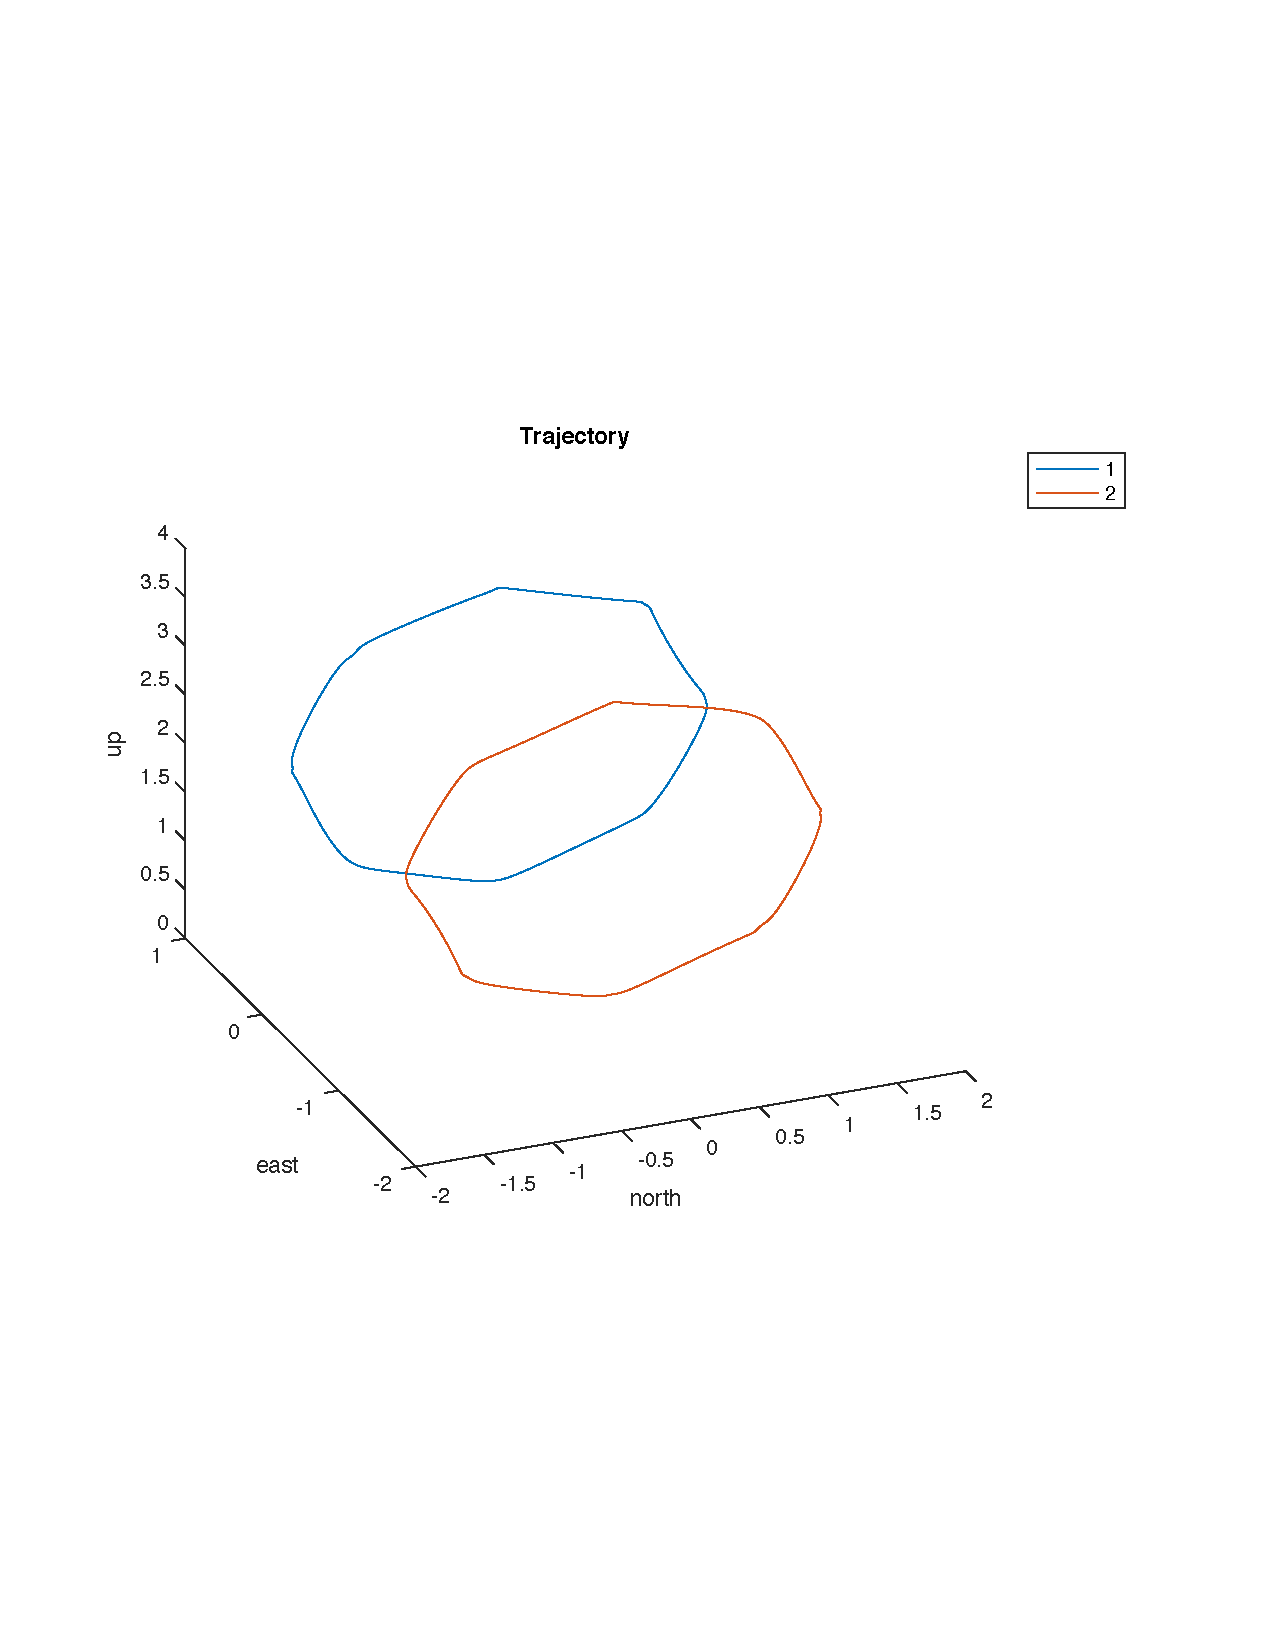
\includegraphics[width=0.7\textwidth]{chapters/chapter-04/figures/trajectory.pdf}
\caption{Trajectory}
\label{fig:trajectory}
\end{figure}

Both the drones start in the upper point of their circle and then they move along the
trajectory in opposite directions. The mission terminates when both the drones reach
their starting point.
The evolution of the trajectory during time of the first drone can be seen in the figure
\ref{fig:trajectory_during_time}.

\begin{figure}
\centering
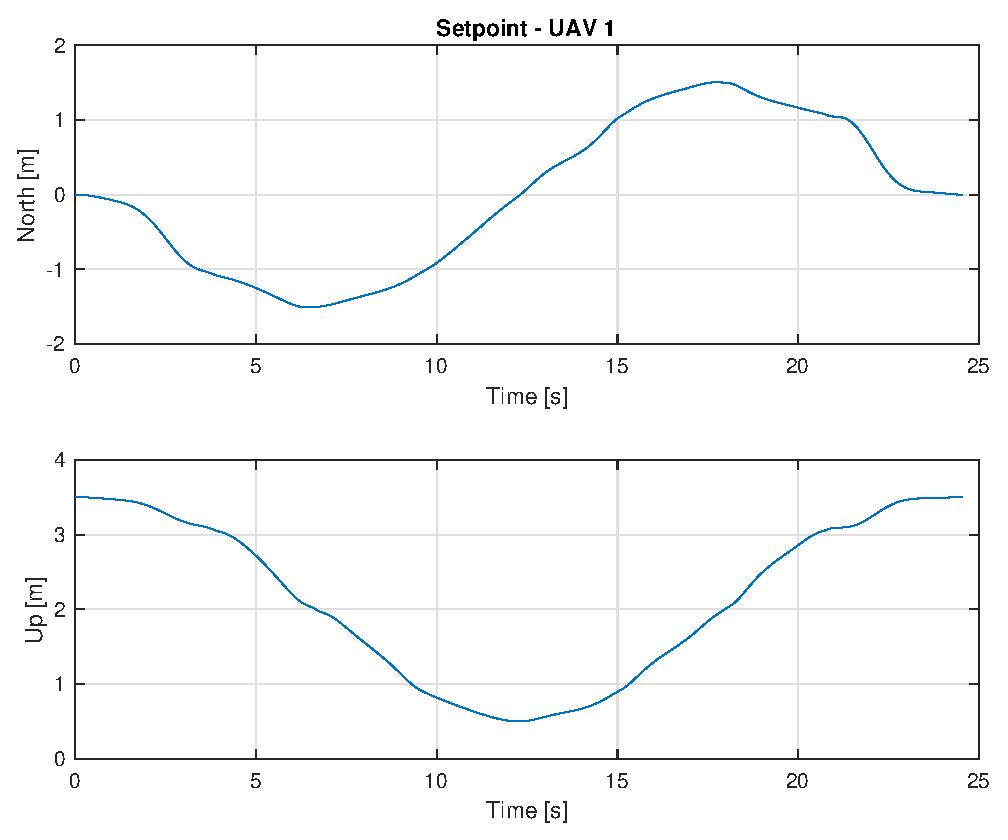
\includegraphics[width=0.7\textwidth]{chapters/chapter-04/figures/pos.eps}
\caption{Evolution of the trajectory during time of the first drone}
\label{fig:trajectory_during_time}
\end{figure}

Now we can see how the two drones follow their trajectory. It is shown in the figures
\ref{fig:following_1} and \ref{fig:following_2}.

\begin{figure}
\centering
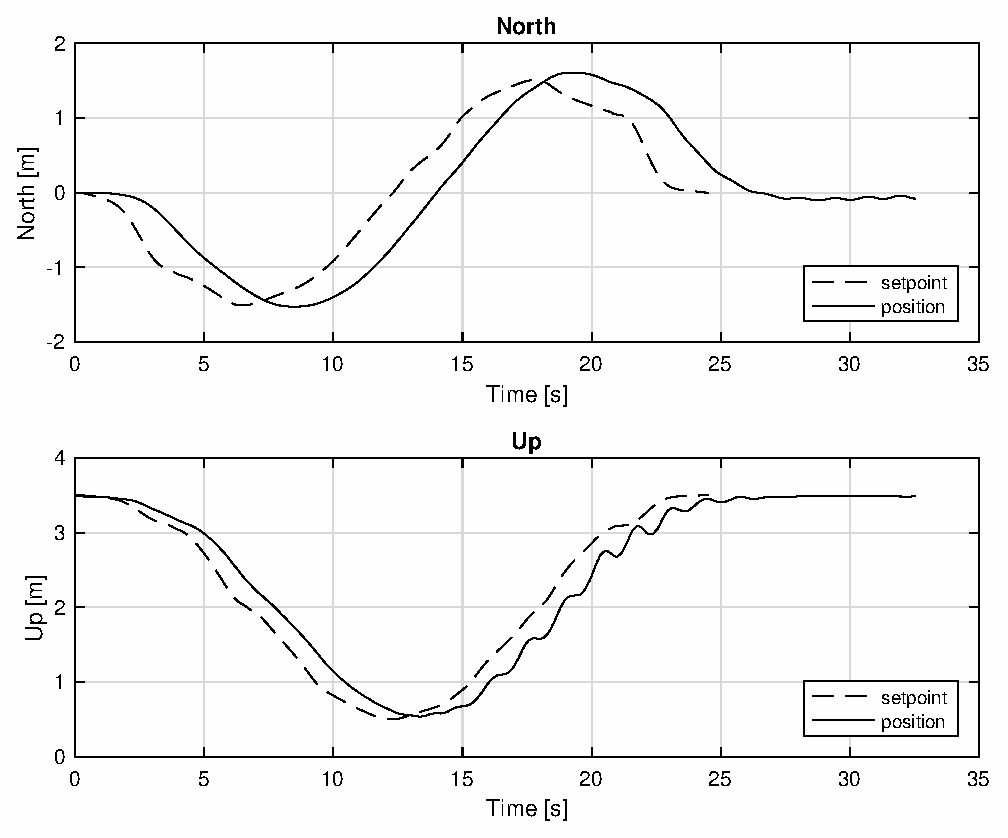
\includegraphics[width=0.7\linewidth]{chapters/chapter-04/figures/following_1.eps}
\caption{Target following drone 1}
\label{fig:following_1}
\end{figure}

\begin{figure}
\centering
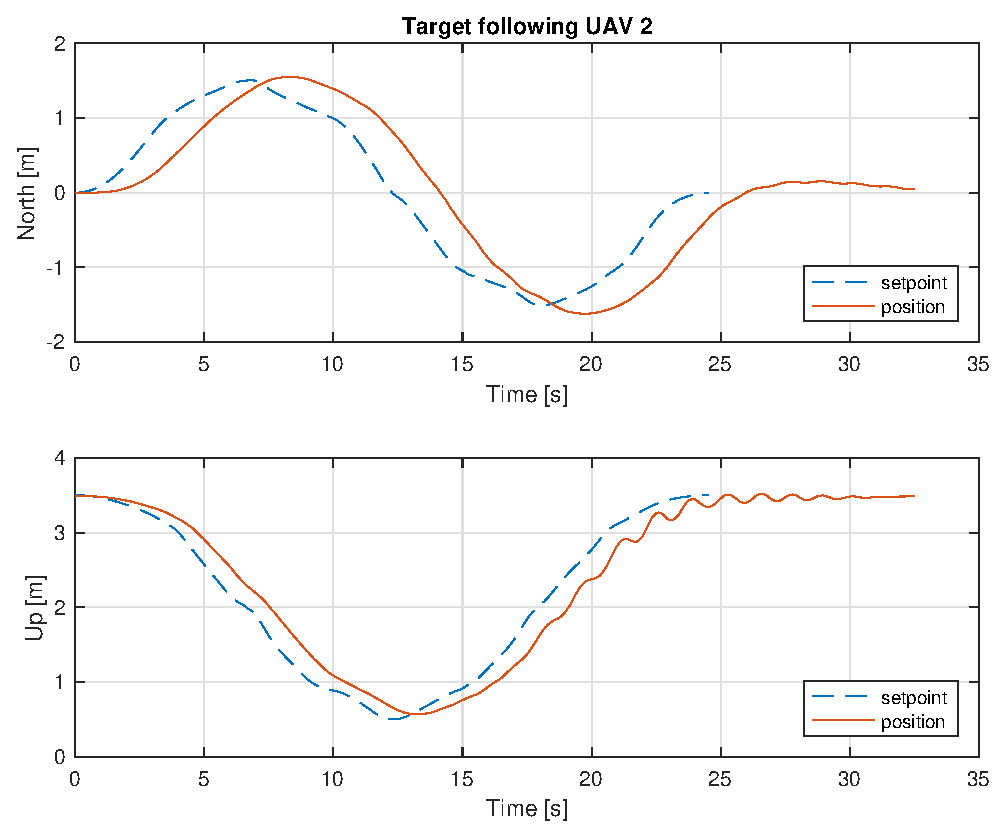
\includegraphics[width=0.7\linewidth]{chapters/chapter-04/figures/following_2.eps}
\caption{Target following drone 2}
\label{fig:following_2}
\end{figure}

There are some delays due to the time needed to the autopilot to follow
the target, but the drones are capable of doing that.
Indeed, they arrive at the same time in their final position.

\begin{figure}
\centering
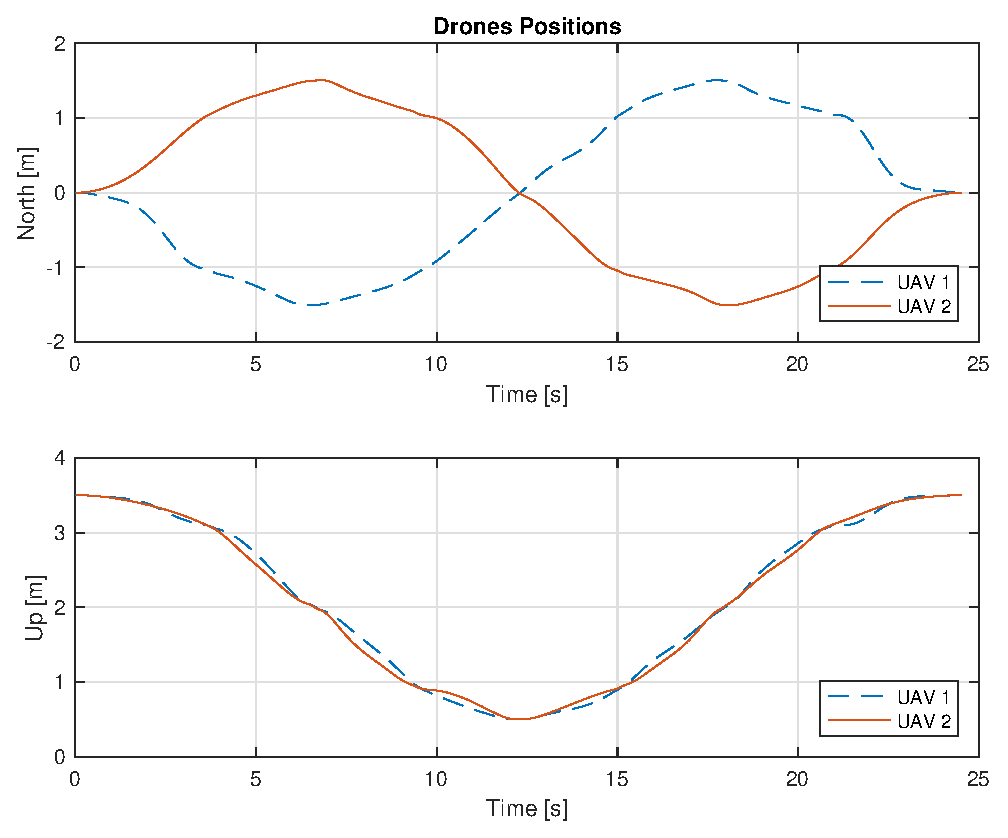
\includegraphics[width=0.7\textwidth]{chapters/chapter-04/figures/overlapped.eps}
\caption{Two drones positions over time}
\label{fig:overlapped}
\end{figure}

If we also consider the figure \ref{fig:overlapped}, we can see that both the drones
are synchronized during the execution of the mission. In the next cases, we will
add disturbances in order to make more evident the effects of the algorithm.


\section{First disturbance}
In this scenario, we use the same trajectory as before (figure \ref{fig:trajectory}),
but in this case we stop one of the two drones and the other will follow it.
We can show the disturbance applied at time 11s to the first drone in the figure \ref{fig:disturbance}.

\begin{figure}
\centering
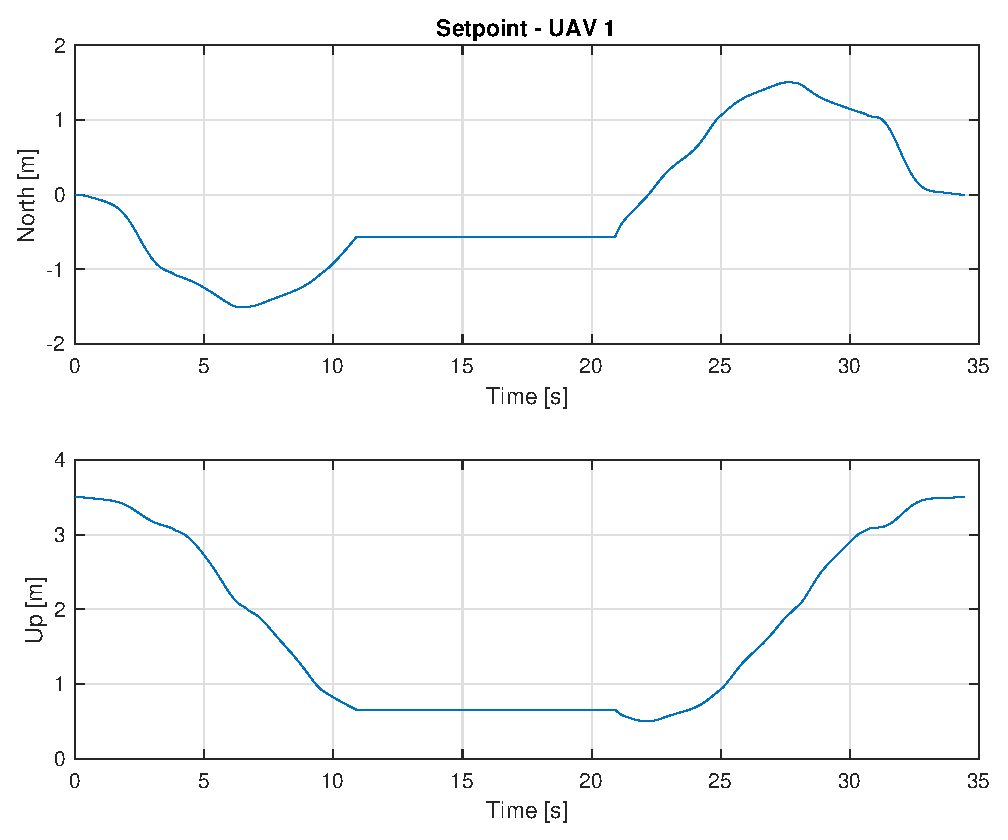
\includegraphics[width=0.7\textwidth]{chapters/chapter-04/figures/pos_1.eps}
\caption{Disturbance}
\label{fig:disturbance}
\end{figure}

We can now see how the two drones execute the mission. The second drone tries to
go on, when the first is interrupted, but then the consensus stops it. The plots are
shown in the figures \ref{fig:following_1_1} and \ref{fig:following_2_1}.

\begin{figure}
\centering
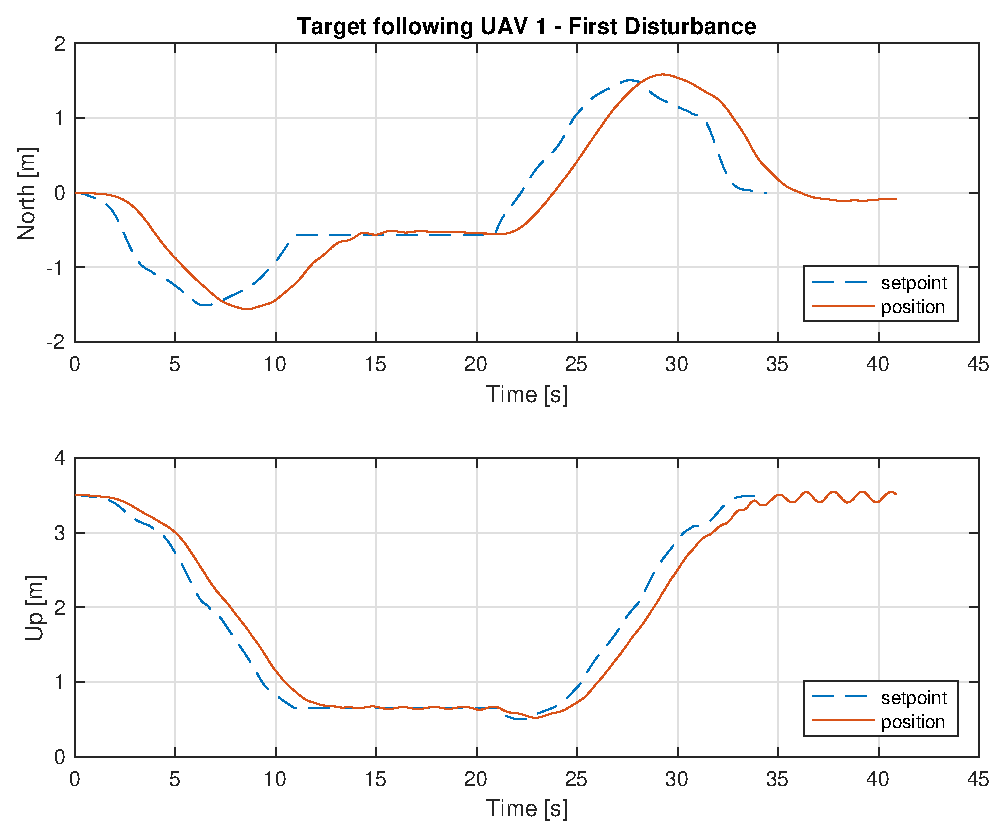
\includegraphics[width=0.7\linewidth]{chapters/chapter-04/figures/following_1_1.eps}
\caption{Target following drone 1}
\label{fig:following_1_1}
\end{figure}

\begin{figure}
\centering
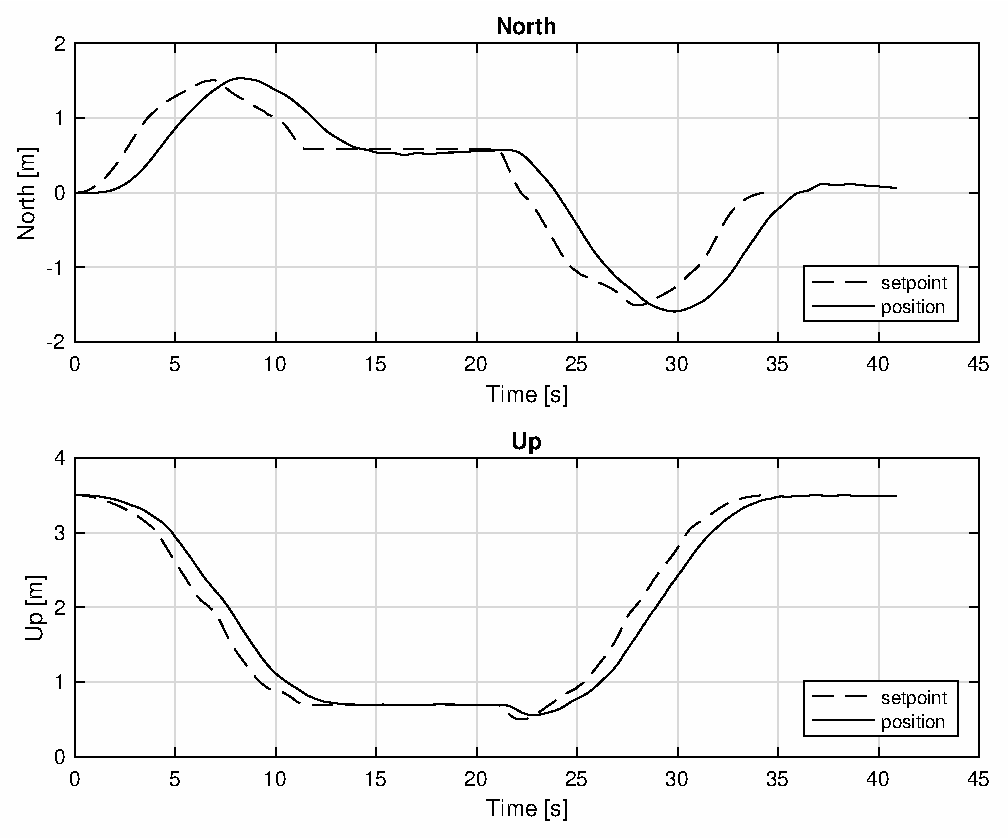
\includegraphics[width=0.7\linewidth]{chapters/chapter-04/figures/following_2_1.eps}
\caption{Target following drone 2}
\label{fig:following_2_1}
\end{figure}

At the end we represent a graph in which we plot the positions of the two drones overlapped
(figure \ref{fig:overlapped_1}).

\begin{figure}
\centering
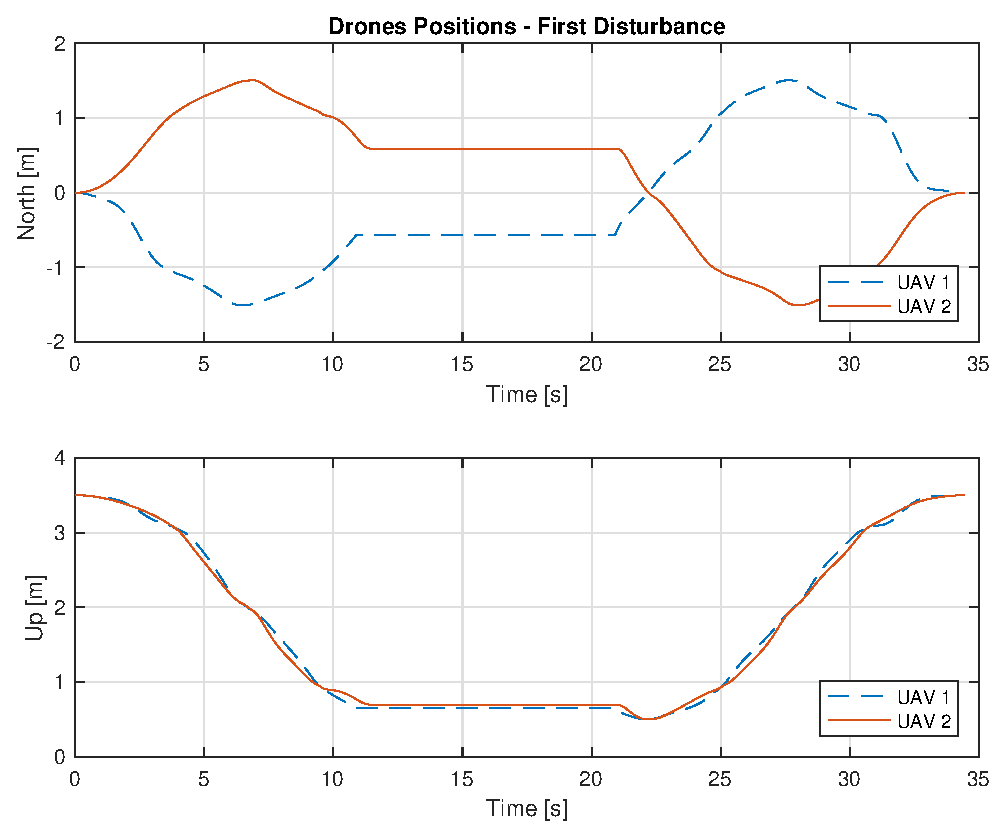
\includegraphics[width=0.7\textwidth]{chapters/chapter-04/figures/overlapped_1.eps}
\caption{Two drones positions over time}
\label{fig:overlapped_1}
\end{figure}


\section{Second disturbance}
The trajectory used is always the same (figure \ref{fig:trajectory}), but this time
the disturbance is different. Now we force one drone to go back through the trajectory
which has travelled so far.
After the disturbance, the drone can resume the trajectory and complete the mission.
We can see the effect of the disturbance on the trajectory in the figure \ref{fig:disturbance_2}.

\begin{figure}
\centering
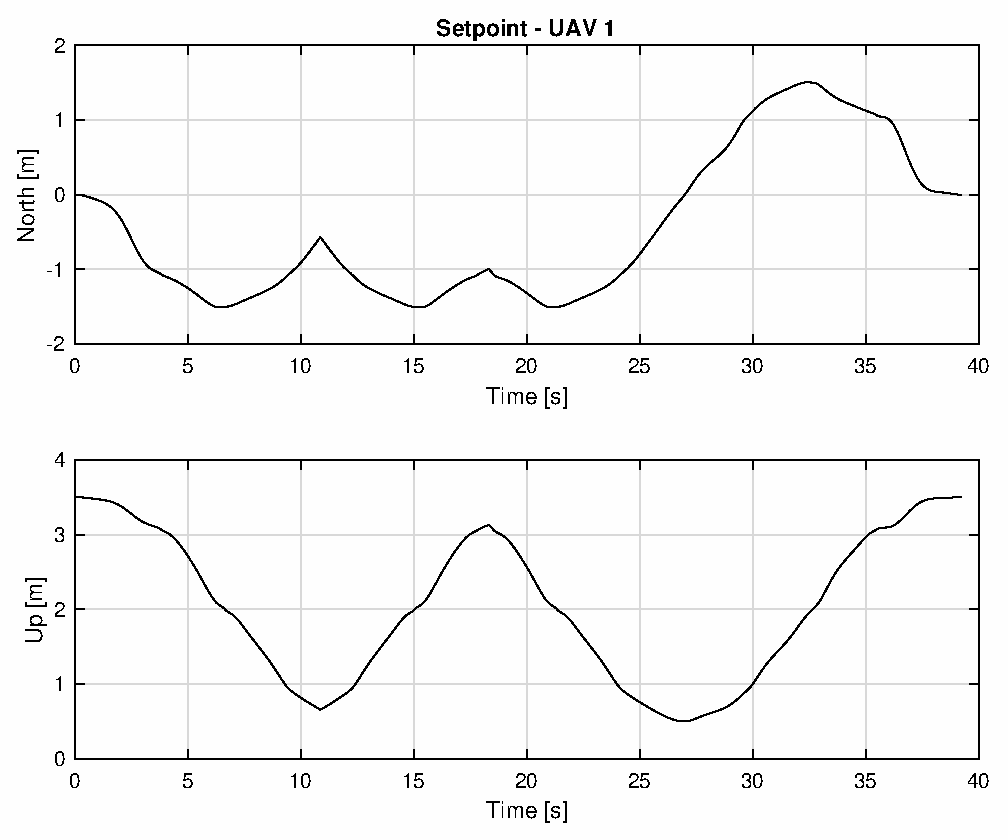
\includegraphics[width=0.7\textwidth]{chapters/chapter-04/figures/pos_2.eps}
\caption{Disturbance}
\label{fig:disturbance_2}
\end{figure}

At time 11s the disturbance starts and the drone start to go back. At time 26s,
the drone is returned to the position where the disturbance is started.

In this situation, the other drone recognizes that the other machine is going back
for an unknown reason and it starts to follow it. We can see how the mission is done
by the two drones in the pictures \ref{fig:following_1_2} and \ref{fig:following_2_2}.

\begin{figure}
\centering
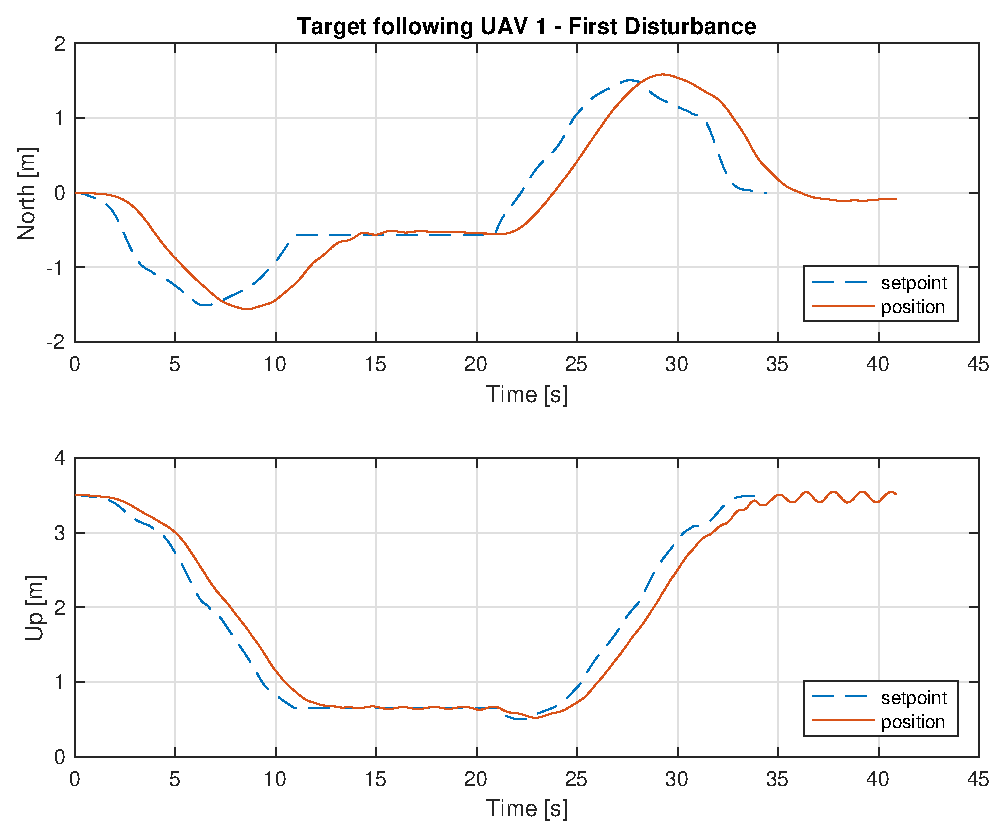
\includegraphics[width=0.7\linewidth]{chapters/chapter-04/figures/following_1_1.eps}
\caption{Target following drone 1}
\label{fig:following_1_2}
\end{figure}

\begin{figure}
\centering
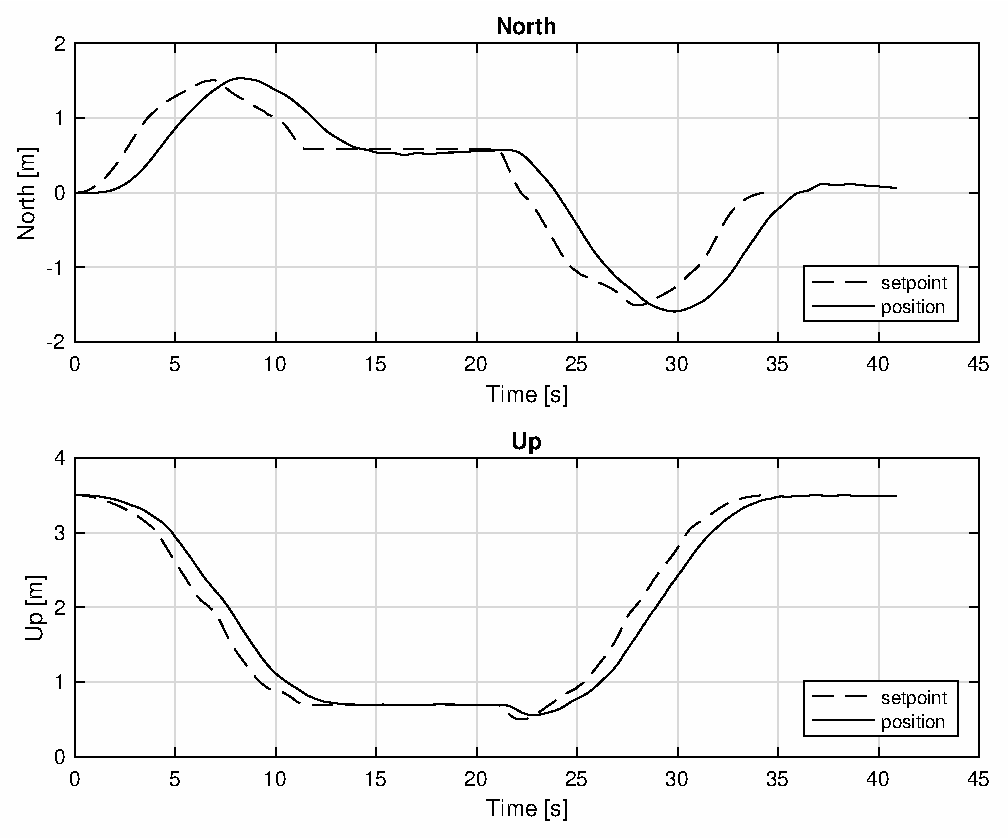
\includegraphics[width=0.7\linewidth]{chapters/chapter-04/figures/following_2_1.eps}
\caption{Target following drone 2}
\label{fig:following_2_2}
\end{figure}

At the end we represent a graph in which we plot the positions of the two drones overlapped
(figure \ref{fig:overlapped_2}).

\begin{figure}
\centering
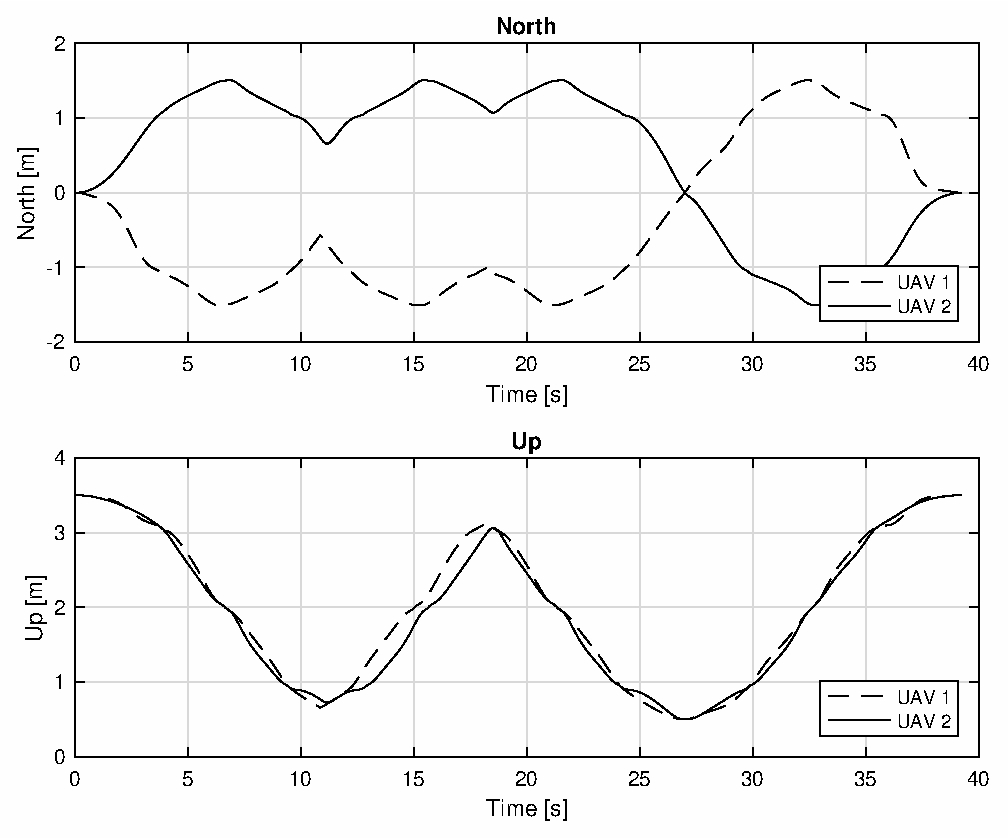
\includegraphics[width=0.7\textwidth]{chapters/chapter-04/figures/overlapped_2.eps}
\caption{Two drones positions over time}
\label{fig:overlapped_2}
\end{figure}


%%%%%%%%%%%%%%%%%%%%%%%%%%%%%% Chapter 10
\chapter{Experimental results\label{chap:experimental_results}}
In this chapter we present the results obtained applying the simulations done in the
previous chapter to a real system.

We want to highlight that the algorithm works even in the real system
and the results obtained are compatible with the simulated ones.
In this scenario, we need to take into account that the network is not ideal and
the data may suffer delays and inaccuracy due to the different clock synchronization
of the machines involved in the experiment.

As in the chapter \ref{chap:simulation_results}, we will run the experiment three times.
First, the formation has to simply follow the trajectory without disturbances.
The second time, we run the algorithm and then we stop one of the drones. The other
will try to go on, but then it stops.
Third, we apply a disturbance which forces one of the drones to go back following
in the reverse order its trajectory. The other drone just follows it, because it is
forced to preserve the formation.

The trajectory used is the same as the simulated one (\ref{fig:trajectory}), and
the drones start on the top points of their trajectory, following the circle in opposite
directions.
They must be symmetric and finish the mission at the same time.

We now present the three cases in detail.

\section{Trajectory following}
The two drones will follow the trajectory, as shown in the figures \ref{fig:exp_following_1}
and \ref{fig:exp_following_2}.

\begin{figure}
\centering
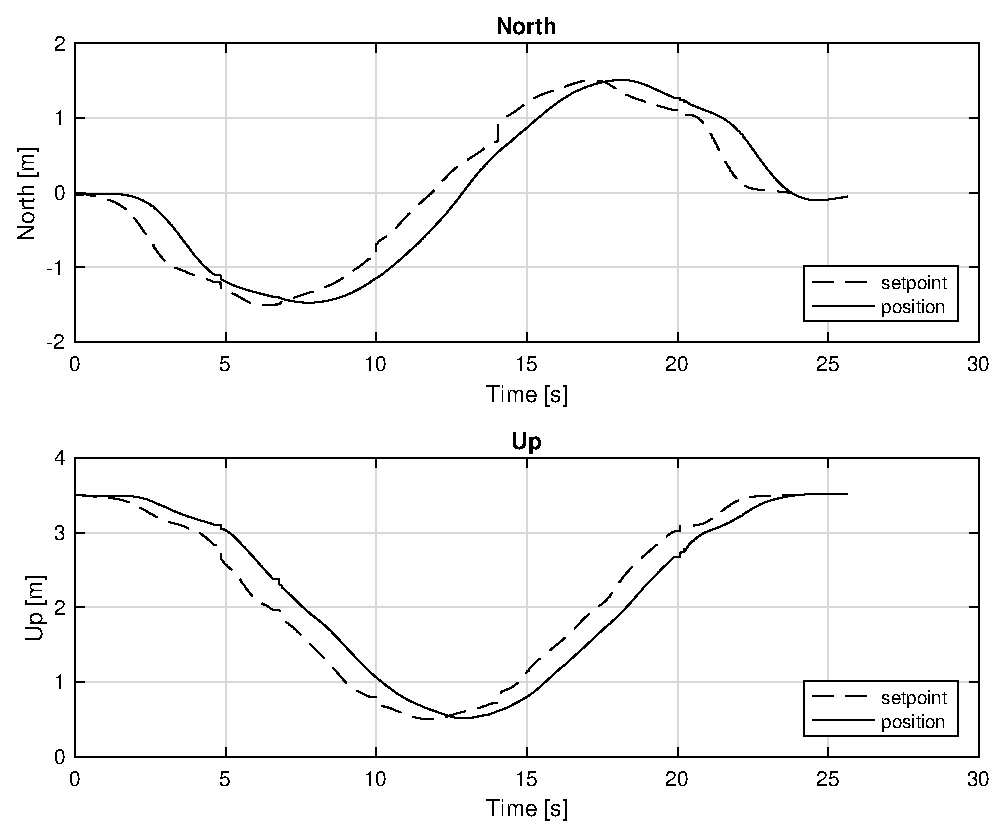
\includegraphics[width=0.7\linewidth]{chapters/chapter-05/figures/following_1.eps}
\caption{Target following drone 1}
\label{fig:exp_following_1}
\end{figure}

\begin{figure}
\centering
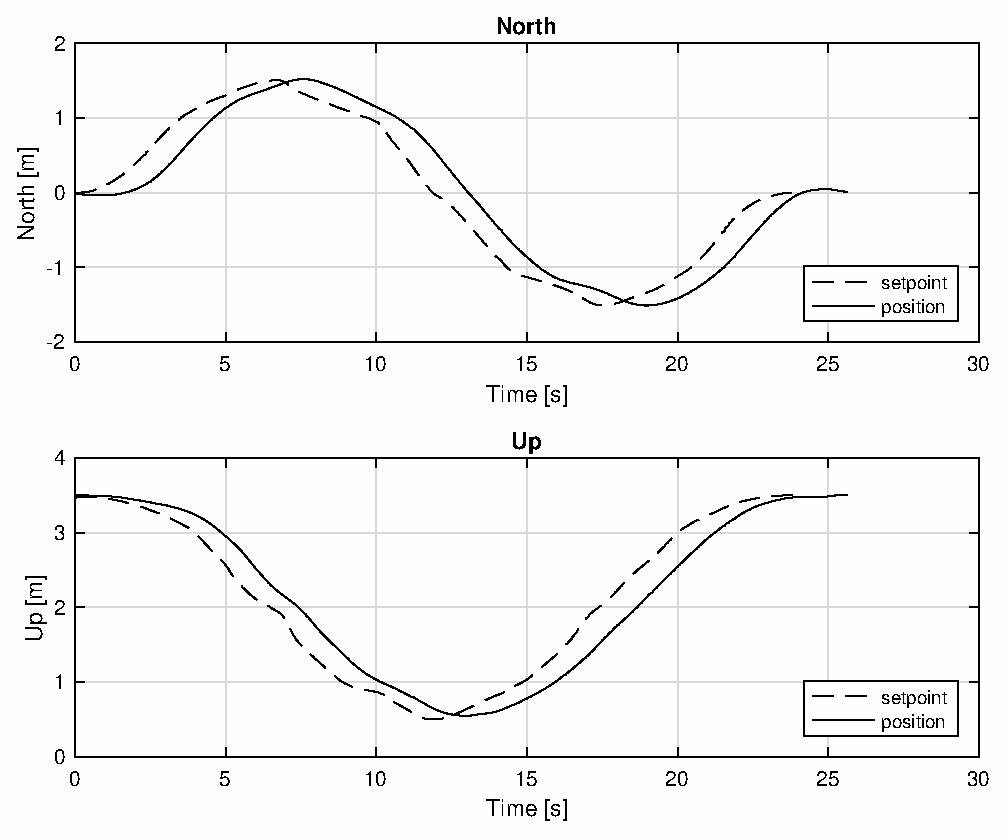
\includegraphics[width=0.7\linewidth]{chapters/chapter-05/figures/following_2.eps}
\caption{Target following drone 2}
\label{fig:exp_following_2}
\end{figure}

Even in this case, there are some delays due to the time needed to the autopilot to follow
the target, but the drones are capable of doing that.
The two drones stay synchronized during all the mission as we can see in the figure
\ref{fig:exp_overlapped}.

\begin{figure}
\centering
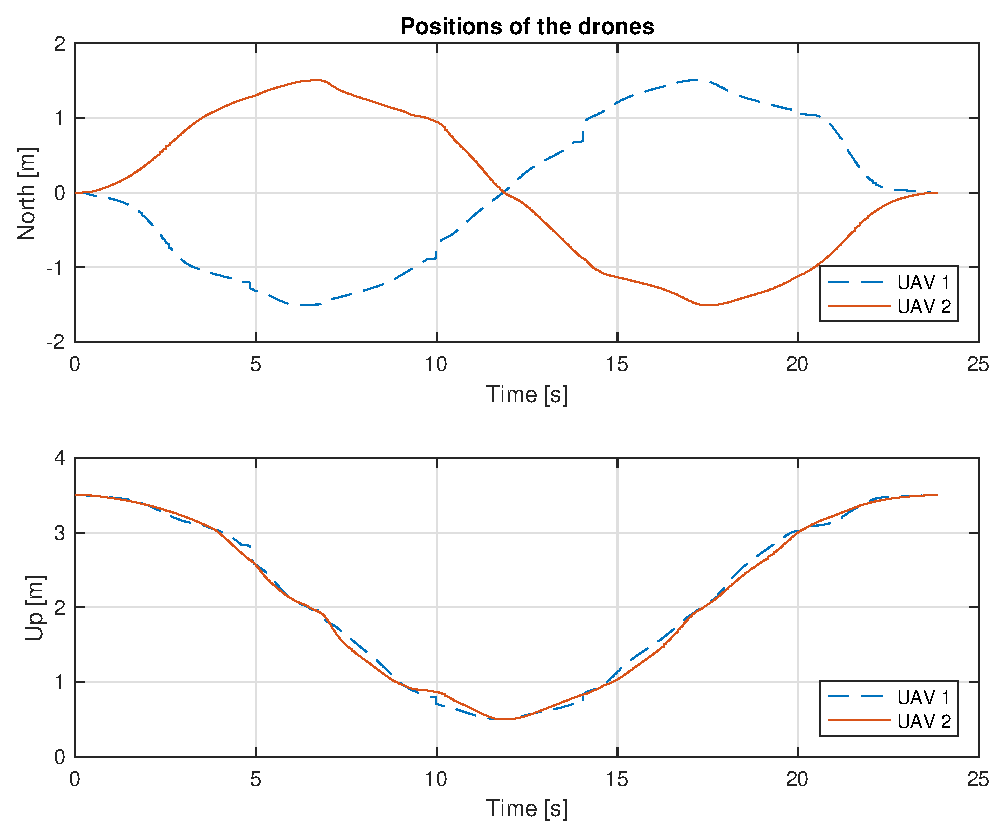
\includegraphics[width=0.7\textwidth]{chapters/chapter-05/figures/overlapped.eps}
\caption{Two drones positions over time}
\label{fig:exp_overlapped}
\end{figure}


\section{First disturbance}

When we add a disturbance to one of the drones, the algorithm rejects it and preserves
the formation. In this experiment we introduce the disturbance a time 6s and it
terminates after 10s. We see the mission in the figures \ref{fig:exp_following_1_1}
and \ref{fig:exp_following_2_1}.

\begin{figure}
\centering
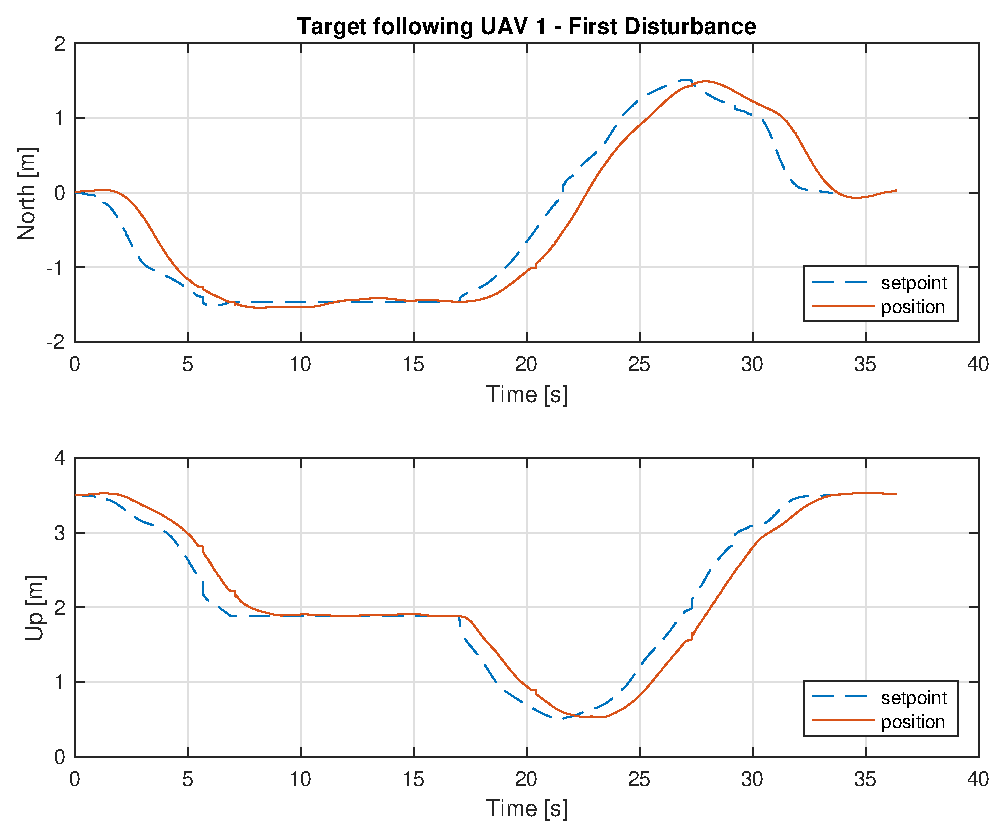
\includegraphics[width=0.7\linewidth]{chapters/chapter-05/figures/following_1_1.eps}
\caption{Target following drone 1}
\label{fig:exp_following_1_1}
\end{figure}

\begin{figure}
\centering
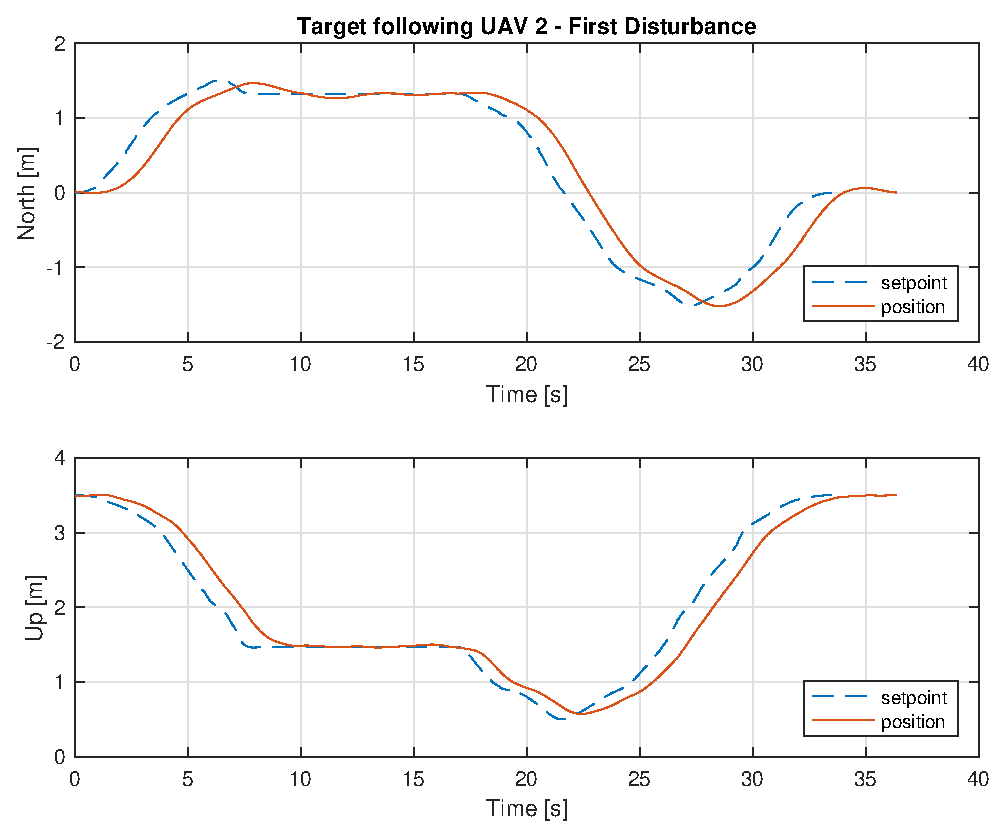
\includegraphics[width=0.7\linewidth]{chapters/chapter-05/figures/following_2_1.eps}
\caption{Target following drone 2}
\label{fig:exp_following_2_1}
\end{figure}

The disturbance causes the other drone to stop and wait until the disturbance
is finished. We can see the synchronization in the figure \ref{fig:exp_overlapped_1}.

\begin{figure}
\centering
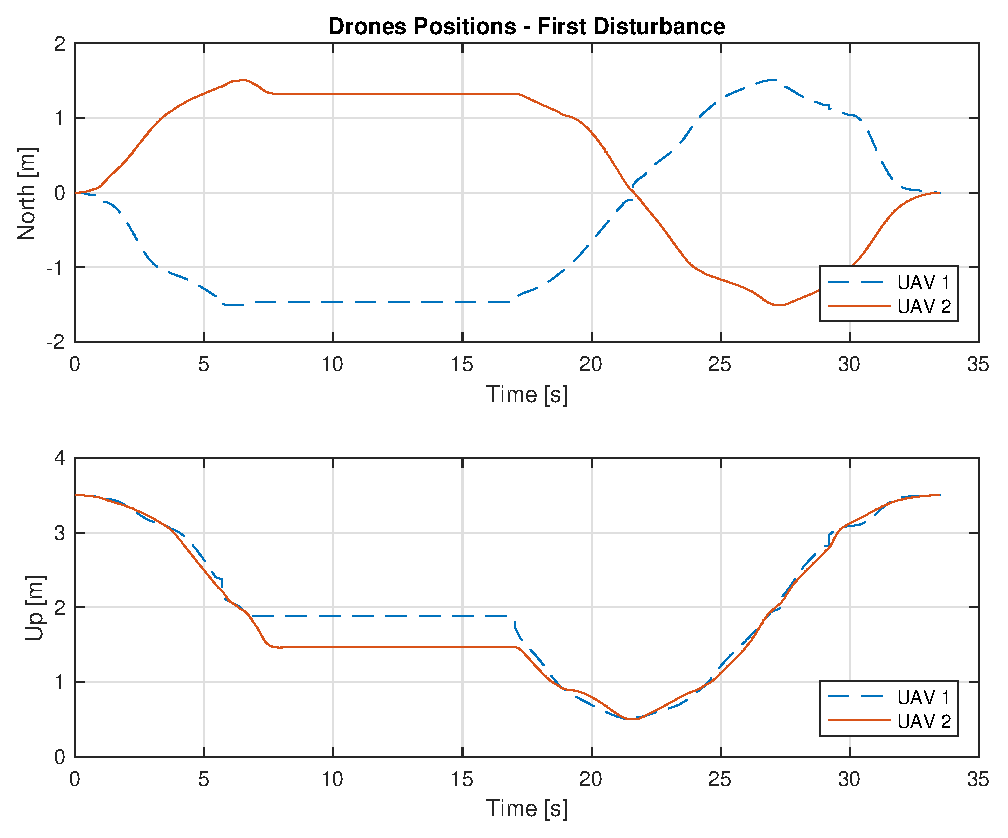
\includegraphics[width=0.7\textwidth]{chapters/chapter-05/figures/overlapped_1.eps}
\caption{Two drones positions over time}
\label{fig:exp_overlapped_1}
\end{figure}

\section{Second disturbance}
The last disturbance we show is the one which forces a drone to go back through the
trajectory. We can see how the setpoints are changed when the disturbance is active
and how the drones follow them. The figures \ref{fig:exp_following_1_2}
and \ref{fig:exp_following_2_2} present the results.

\begin{figure}
\centering
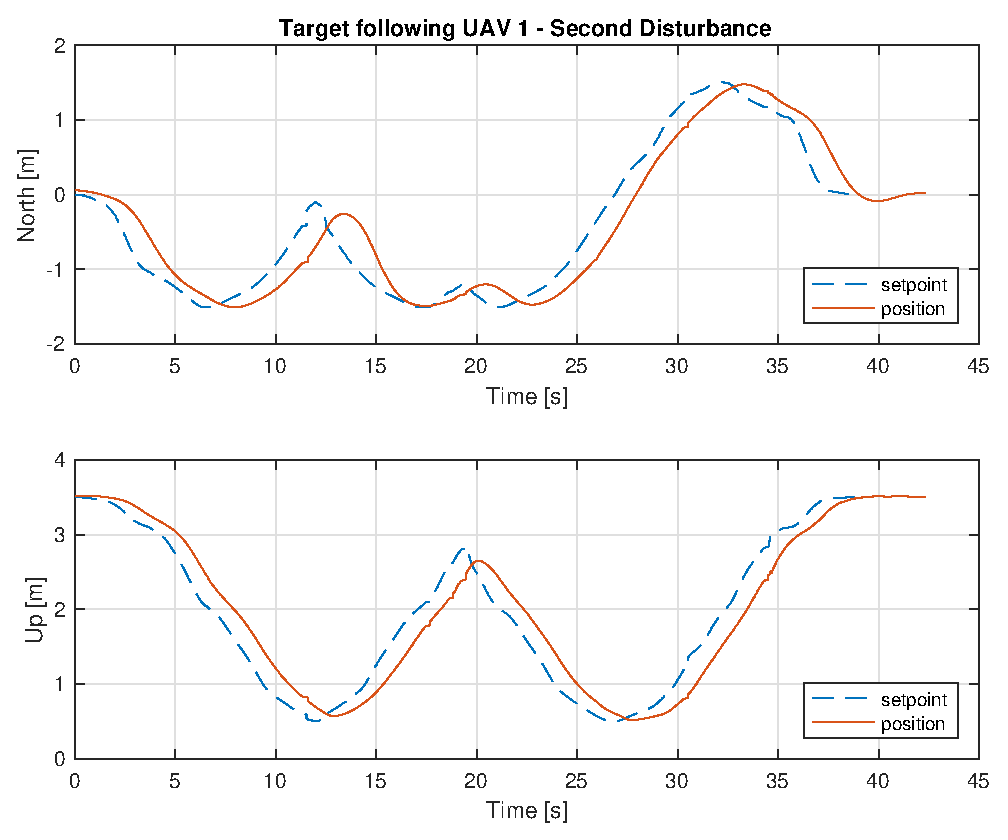
\includegraphics[width=0.7\linewidth]{chapters/chapter-05/figures/following_1_2.eps}
\caption{Target following drone 1}
\label{fig:exp_following_1_2}
\end{figure}

\begin{figure}
\centering
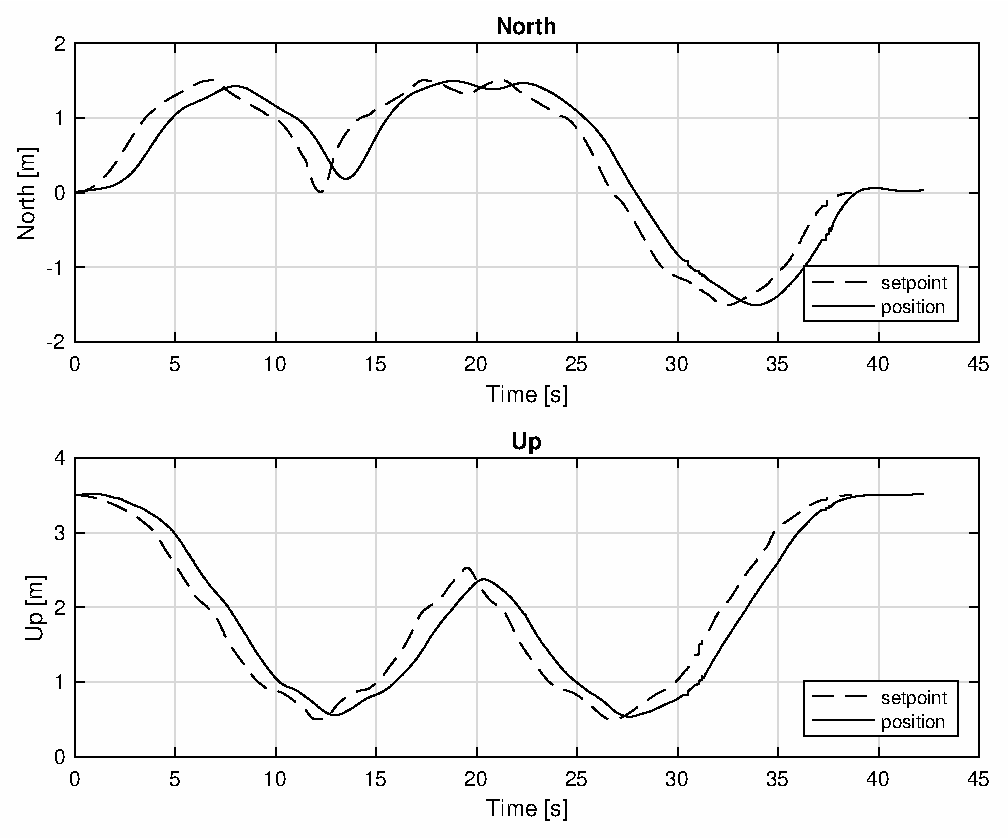
\includegraphics[width=0.7\linewidth]{chapters/chapter-05/figures/following_2_2.eps}
\caption{Target following drone 2}
\label{fig:exp_following_2_2}
\end{figure}

The disturbance causes the other drone to stop and go back, following the other,
until the disturbance is finished.
We can see the synchronization in the figure \ref{fig:exp_overlapped_2}.

\begin{figure}
\centering
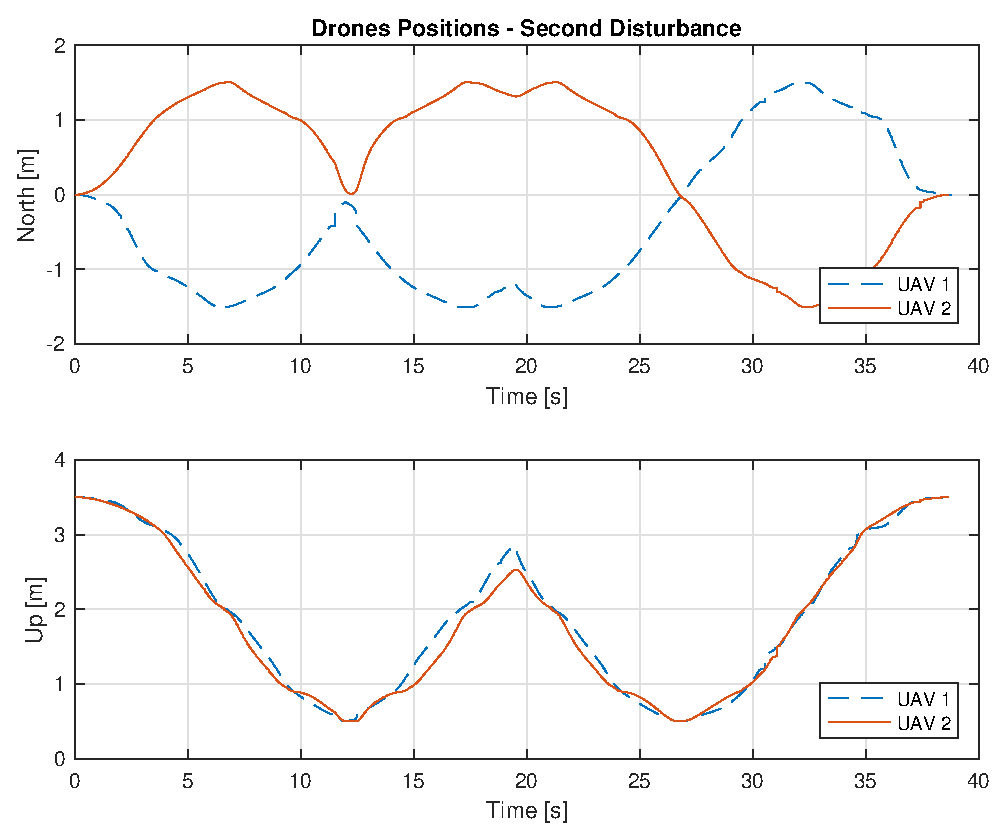
\includegraphics[width=0.7\textwidth]{chapters/chapter-05/figures/overlapped_2.eps}
\caption{Two drones positions over time}
\label{fig:exp_overlapped_2}
\end{figure}

The experimental results are less accurate than the simulated ones,
but the overall behaviour is preserved.


%%%%%%%%%%%%%%%%%%%%%%%%%%%%%% Conclusion
\chapter*{Conclusions}
\addcontentsline{toc}{chapter}{Conclusions}
\markboth{Conclusions}{Conclusions}
%The conclusions must recall the field of work, the purpose of the thesis, what has been done and an evaluation of the obtained results.
%Furthermore, the conclusion must also emphasize the future prospects and must show how to move forward in the study area.

The results obtained in our experiments can be applied in many fields in which
a formation of UAVs has to operate.
In this thesis, we have shown how the consensus algorithm is deployed on a real
system and which performances can be achieved.

The implementation allows us to plan and fulfill a cooperative
mission in which the synchronization is one of the most important aspects.
The system is robust to network delays and loss of packets and to unexpected failures
of the vehicles involved.
Moreover, the formation, if equipped with an obstacle avoidance algorithm,
overcomes the presence of unexpected obstacles during the execution of the mission.

Further studies can be carried on in order to integrate recovery procedures in case
of network failures or the loss of a machine.
It is possible to develop obstacle avoidance algorithms or any kind of online procedures
acting directly on the free parameters of the algorithm presented.
In particular, it is possible to change the values of $\ddot{\gamma_d}$ and $\dot{\gamma_d}$,
in order to modify the velocity of the execution of the mission. These two values
can be also used to build more complex functionalities on top of the consensus algorithm.


%%%%%%%%%%%%%%%%%%%%%%%%%%%%%% Bibliography
\bibliographystyle{plain}
\bibliography{bibliography}

%%%%%%%%%%%%%%%%%%%%%%%%%%%%%% Appendix A
\appendix
\chapter{First appendix\label{app:first-appendix}}



%%%%%%%%%%%%%%%%%%%%%%%%%%%%%% Appendix B
\chapter{Second appendix\label{app:second-appendix}}



%%%%%%%%%%%%%%%%%%%%%%%%%%%%%% Appendix  C
\chapter{Third appendix\label{app:third-appendix}}


\cleardoublepage{}

%%%%%%%%%%%%%%%%%%%%%%%%%%%%%% END OF THE DOCUMENT
\end{document}
